% --------------------------------------------------------------------------------------
%% Canevas pour le mémoire de Master 2 TNAH - ENC (10/08/2020)
%% main.tex
%% Copyright 2020 L. Terriel (lucas.terriel@chartes.psl.eu / ls.terriel@gmail.com)
% --------------------------------------------------------------------------------------
% Ce(tte) œuvre est mise à disposition selon les termes de la Licence Creative Commons :
%% - Attribution 
%% - Pas d’Utilisation Commerciale 
%% - Partage dans les Mêmes Conditions 4.0 International.
% --------------------------------------------------------------------------------------
% Ce fichier fait partie d'un ensemble de fichiers .tex 
% appartenant au projet LaTeX "L-TERRIEL_memoireDeStage_M2TNAH_ENC"
% --------------------------------------------------------------------------------------

\documentclass[a4paper, twoside, 12pt]{book}

\usepackage[french]{babel}

%--------------------------
% INPUTENC (encodage du texte)
% FONTENC (positionnement des accents)
%--------------------------
\usepackage[utf8]{inputenc}
\usepackage[T1]{fontenc}
%--------------------------
% HYPERREF (liens hypertextes et métadonnées)
%--------------------------
\usepackage{hyperref}
\hypersetup{
colorlinks=true,
linkcolor=black,
urlcolor=blue,
citecolor=black
}

\title{Mémoire de Master 2 Technologies numériques appliqués à l'histoire - Ecole nationale des chartes - 2020}
\author{Lucas Terriel}

%--------------------------
% TOCBIBIND (ajouter la bibliographie dans la Table des matières)
%--------------------------
\usepackage{tocbibind}

%--------------------------
% Éléments de mise en page (marge de 2,5 cm, alinéa en début de paragraphe 1cm, interligne 1,5)
%--------------------------
\usepackage[a4paper, margin=2.5cm]{geometry}
\usepackage{setspace}
\onehalfspacing
\setlength{\parindent}{1cm}

\usepackage{fancyhdr}
\renewcommand{\chaptermark}[1]{\markboth{#1}{}}
\renewcommand{\sectionmark}[1]{\markright{#1}}
\pagestyle{fancy}
\fancyhf{}
\renewcommand{\chaptermark}[1]{\markboth{\bsc{\chaptername~\thechapter{} :} #1}{}}
\renewcommand{\sectionmark}[1]{\markright{\thesection{} \ #1}}
\renewcommand{\headrulewidth}{0pt}
\lhead[]{\textsl{\rightmark}}
\rhead[\textsl{\leftmark}]{}
\cfoot[\thepage]{\thepage}

%--------------------------
% Mise en page des tableaux
%--------------------------

% pour les longs tableaux
\usepackage{longtable}
% longueur / largeur :
\usepackage{chngpage}
% paysage :
\usepackage{lscape} 
% couleurs
\usepackage{colortbl}

%--------------------------
% Modules pour gérer les listes
%--------------------------
\usepackage{enumerate}
\usepackage{enumitem}

%--------------------------
% Modules pour créer des arborescences 
%--------------------------
\usepackage{dirtree}

%-------------------------
% Modules pour citer du code (LISTING)
%-------------------------
\usepackage{listings}
\usepackage{xcolor}

\definecolor{dkgreen}{RGB}{112,211,98}
\definecolor{gray}{rgb}{0.5,0.5,0.5}
%\definecolor{mauve}{rgb}{0.58,0,0.82}
\definecolor{orange}{RGB}{229,148,0}
%\definecolor{lightblue}{RGB}{50,162,223}
%\definecolor{brickred}{RGB}{206,28,9}
\definecolor{dkblue}{RGB}{71,118,105}
\definecolor{lightgray}{RGB}{251,252,251}

\lstset{%
backgroundcolor=\color{lightgray},
frameround=fttt,
aboveskip=3mm,
belowskip=3mm,
showstringspaces=false,
columns=flexible,
basicstyle={\small\ttfamily},
numbers=left,
numberstyle=\tt\tiny\color{gray},
keywordstyle=\color{dkblue},
commentstyle=\color{dkgreen},
stringstyle=\color{orange},
breaklines=true,
breakatwhitespace=true,
tabsize=3
}

%--------------------------
% GESTION DE LA BIBLIOGRAPHIE
%--------------------------
\usepackage[backend=biber, sorting=nyt, style=enc]{biblatex}
\usepackage[autostyle]{csquotes}

%\bibliography{bibliographie.bib}
\addbibresource{bibliographie.bib}

%--------------------------
% COMMANDES ET ENVIRONNEMENTS PERSONNALISÉS
%--------------------------
\newcommand{\hugeskip}{\bigskip \bigskip \bigskip}
\newcommand{\citecode}[1]{\texttt{\textmd{#1}}}
\newcommand{\inquote}[1]{\og{}#1\fg{}}
\newcommand{\lgS}{\char"017F}

\setcounter{secnumdepth}{5}
\setcounter{tocdepth}{3}

\usepackage[official]{eurosym}
\usepackage{afterpage}

%--------------------------
% FIGURES
%--------------------------
\usepackage{graphicx}
\graphicspath{ {./images/} }
\usepackage{float}
\usepackage{wrapfig}
\usepackage{subcaption}
\usepackage{minted}
\usepackage{lscape}
\usepackage{rotating}
\usepackage{listings}

\usepackage{float}

%---------------------------
% SYMBOLES
%---------------------------
\usepackage{eurosym}



% ============================================

\begin{document}

% Pour les parties réglementaires : 
\frontmatter
\begin{titlepage}
    \begin{center}

        \bigskip
    
        \begin{large}
            \'ECOLE NATIONALE DES CHARTES 
        \end{large}
    
        \begin{center}
            \rule{4cm}{0.02cm}
        \end{center}
    
        \hugeskip
        
        \begin{Large}
             \textbf{Lucas Terriel}\\
        \end{Large}
        \begin{normalsize}
            \textit{Licencié ès histoire}\\
            \textit{Diplômé de master 
            Histoire, Civilisations, Patrimoine contemporains}\\
        \end{normalsize}
        
        \hugeskip
        \bigskip
        
        % informations à compléter
        \begin{LARGE}
            \textbf{Représenter et évaluer les données issues de la structuration et de la transcription automatique d'un corpus.}
            
        \end{LARGE}
        \bigskip
        \bigskip
        \bigskip
        \bigskip
        \begin{large}
            \textbf{L'exemple de la reconnaissance automatique des écritures manuscrites sur les répertoires de notaires du projet Lectaurep.}\\
        \end{large}
        
        \hugeskip
        \vfill
        
        
        
        \begin{large}
            Mémoire pour le diplôme\\
            \og Technologies numériques appliquées à l'histoire \fg\\
            \bigskip
            2020
        \end{large}
        
        \begin{figure}[H]
            \centering
            
\includegraphics[width=2.5cm]{cc-icon.png}
            \label{traitement}
        \end{figure}
        
    \end{center}
\end{titlepage}

\thispagestyle{empty}
\cleardoublepage
        \begin{figure}[H]
            \centering
            
\includegraphics[width=3cm]{cc-icon.png}
            \label{traitement}
        \end{figure}

    Ce mémoire professionnel/recherche est placé sous les termes de la licence Creative Commons en ces termes : \textbf{Attribution - Pas d'Utilisation Commerciale - Partage dans les Mêmes Conditions 4.0 International (CC BY-NC-SA 4.0)}.
\bigskip

    Consulter la \href{https://creativecommons.org/licenses/by-nc-sa/4.0/legalcode.fr}{licence\footnote{%
\textit{Licence CC 4.0 International}, en ligne: <\url{https://creativecommons.org/licenses/by-nc-sa/4.0/legalcode.fr}>.}} en entier pour plus de détails. 
\bigskip

    Vous êtes autorisé à :
    \begin{itemize}
        \item \textbf{Attribution} : Vous devez créditer l'\oe uvre, intégrer un lien vers la licence et indiquer si des modifications ont été effectuées à l'\oe uvre. Vous devez indiquer ces informations par tous les moyens raisonnables, sans toutefois suggérer que l'Offrant vous soutient ou soutient la façon dont vous avez utilisé son \oe uvre;
        \item \textbf{Pas d'utilisation commerciale} : Vous n'êtes pas autorisé à faire un usage commercial de cette \oe uvre, tout ou partie du matériel la composant. 
        \item \textbf{Partager — copier, distribuer et communiquer} le matériel par tous moyens et sous tous formats;
        \item \textbf{Adapter — remixer, transformer et créer} à partir du matériel.
    \end{itemize}
\bigskip

L'Offrant ne peut retirer les autorisations concédées par la licence tant que vous appliquez les termes de cette licence.


\chapter*{Résumé}
\addcontentsline{toc}{chapter}{Résumé}
\markboth{Résumé}{} 
Ce mémoire a été réalisé en vue de l'obtention du diplôme de Master 2 \inquote{Technologies numériques appliquées à l'histoire} de l'École nationale des chartes. Il a été rédigé à la suite d'un stage de quatre mois au sein de l'équipe ALMAnaCH d'Inria, et dont le déroulé s'est inscrit dans le cadre de Time Us. Ce projet de recherche pluri-institutionnel porte sur l'histoire de l'industrie du textile en France (fin XVII\up{e}-début XX\up{e} siècles) et sur la reconstitution des budget temps des ouvriers et ouvrières du textile. Time Us explore également l'utilisation d'outils informatique pour réaliser cette recherche. 
Ce mémoire étudie le traitement informatique appliqué à une partie du corpus de Time Us, de la structuration à l'éditorialisation. 
Il s'agit d'une analyse critique des enjeux, stratégies et résultats envisagés dans le cadre du projet Time Us autant que du stage, dont le but est de rendre compte d'un exemple de projet et de développement s'inscrivant dans le cadre des humanités numériques.


\bigskip

%informations à compléter
\textbf{Mots-clefs:} TAL; métadonnées; données; format pivot; XML-TEI; développement applicatif; similarité syntaxique; similarité sémantique; métriques \textit{text-to-text}; OCR; HTR; Machine learning; Intelligence artificielle; répertoires de notaires; valorisation patrimoniale; Humanités numériques.

\bigskip
\bigskip
\bigskip

% informations à compléter
\textbf{Informations bibliographiques:} Lucas Terriel, \textit{Représenter et évaluer les données issues de la structuration et de la transcription automatique d'un corpus. L'exemple de la reconnaissance automatique des écritures manuscrites sur les répertoires de notaires du projet Lectaurep.}, mémoire de master \og Technologies numériques appliquées à l'histoire \fg{}, dir. Alix Chagué et Thibault Clérice, École nationale des chartes, 2020.

\clearpage
\thispagestyle{empty}
\cleardoublepage
\chapter*{Remerciements}
\addcontentsline{toc}{chapter}{Remerciements}
\markboth{Remerciements}{} 

Pour ce stage, qui s'est déroulé durant la période de confinement, je tiens à remercier l'ensemble des personnes qui m'ont aidé et soutenu dans cette situation particulière et qui m'ont encouragé dans mon travail.

En premier lieu, je remercie mon tuteur pédagogique, M. Thibault Clérice, et ma tutrice professionnel, Mme Alix Chagué, ingénieure recherche et développement, pour leurs appuis et leurs conseils avisés. 

Je remercie l'ensemble de l'équipe du projet Lectaurep, et le personnel du Minutier central des notaires de Paris aux Archives nationales, Mme Marie-Françoise Limon-Bonnet, responsable du département, Mme Aurélia Rostaing, responsable du pôle instruments de recherche, M. Gaetano Piraino, responsable à la DMOASI, M. Danis Habib, chargé d'études documentaires, Mme Virginie Grégoire, secrétaire de documentation, M. Benjamin Davy, agent technique d'accueil, surveillance et magasinage, et Mme Anna Chéru, stagiaire phase 3. 

Je remercie l'équipe ALMAnaCH d'Inria, qui ont su créer les conditions favorables d'accueil de mon stage et permis un environnement de travail stimulant; je remercie en particulier M. Laurent Romary, directeur de recherche, pour nos échanges et ses conseils pertinents et Mme Florianne Chiffoleau, ingénieure recherche et développement, pour son aide.

Comme le stage est un travail d'équipe avant tout, je remercie Jean-Damien Généro, collègue de master TNAH à l'École nationale des chartes, qui était stagiaire durant la même période à ALMAnaCH sur le projet Time us, dont la mise en commun de nos efforts et nos échanges sur les scripts ont permis le bon déroulement technique et pratique de nos stages respectifs.

Enfin je remercie ma famille et mes amis, pour leurs indéfectible soutient tout au long de cette période. 
\chapter*{Liste des sigles et abréviations}
\addcontentsline{toc}{chapter}{Liste des sigles et abréviations}
\markboth{Liste des sigles abréviations}{} 

\begin{itemize}
    \item A.N. : Archives Nationales
    \item DMC : Département du Minutier central des notaires de Paris  
    \item DMOASI : département de la maîtrise d’ouvrage du système d’information (direction de l’appui scientifique) 
\end{itemize}

\begin{center}
$\star$
\end{center} 

\begin{itemize}
    \item ALMAnaCH : \emph{Automatic Language Modelling and Analysis \& Computational Humanities}
    \item ANR : Agence Nationale de la Recherche
    \item EPI : Équipe-Projet Inria
    \item INRIA : Institut Nationale de Recherche en Informatique et Automatique
    \item LECTAUREP : Lecture automatique des répertoires
    \item W3C : World Wide Web Consortium
\end{itemize}

\begin{center}
$\star$
\end{center} 

\begin{itemize}
    \item EN : Entités Nommées
    \item ML : \emph{Machine Learning}
    \item REN : Reconnaissance d'Entités Nommées
    \item RNN : \emph{Recurrent neural network} - Réseau de neurones récurrents
    \item TAL : Traitement Automatique des Langues
\end{itemize}


\begin{center}
$\star$
\end{center} 

\begin{itemize}
    
    \item CSS : \emph{Cascading Style Sheets}
    \item CSV : \emph{Comma-separated values}
    \item DTD : \emph{Document Type Definition}
    \item HTML : \emph{HyperText Markup Language}
    \item HTR : \emph{Handwritten Text Recognition}
    \item OCR : \emph{Optical Character Recognition}
    \item ODD : \emph{One Document Does it all}
    \item PDF : \emph{Portable Document Format}
    \item RELAXNG : \emph{Regular Language for XML Next Generation}
    \item TEI : \emph{Text Encoding Initiative}
    \item XML : \emph{eXtensible Markup Language}
    \item XSLT : \emph{eXtensible Stylesheet Language Transformations}
\end{itemize}


% Pour les parties principales : 
\mainmatter
\part*{Introduction}
\addcontentsline{toc}{part}{Introduction}
\markboth{Introduction}{Introduction}
\part{Le projet Lectaurep : un cas d'application de l' \og intelligence artificielle\fg{}  aux documents historiques}
\chapter{État de l'art du \textit{machine learning}, de la reconnaissance automatique des écritures manuscrites et de l'implication de ces techniques dans le cadre de projets de traitement automatique du langage (TAL)}
\section{Principes élémentaires du \textit{machine learning}}
\subsection{a voir ?}
\section{La reconnaissance automatique des écritures manuscrites : un domaine entre le traitement automatique du langage (TAL) et le \textit{machine learning}}
\chapter{Lectaurep, un projet de recherche et développement en reconnaissance automatique des écritures manuscrites}
\section{Des origines à la phase 3}
\section{Une dimension expérimentale}
\part{Représenter, enrichir et homogénéiser dans un format pivot les données et métadonnées au sein de la chaîne de traitement Lectaurep}

Objectifs de la mission ? 

\chapter{Enjeux et problématiques liés aux données et aux formats dans le projet}
\section{De l'importance des données et métadonnées}
\section{Les répertoires de notaires ne sont pas que des images numérisées !}
- permettre IIIF

\chapter{Le choix du XML TEI (\textit{Text Encoding Initiative}) comme format pivot}
\section{Un choix réaliste ? le format XML TEI dans d'autres projets et apports pour Lectaurep}
\section{Esquisse d'un format pivot et premières spécifications TEI grâce l'ODD}

\chapter{Simuler la récupération, l'export et la validation d'un format pivot XML TEI}
\section{Objectifs et buts de la simulation}
- ne parle forcément aux archivistes;
- besoin de visualiser les données dans un canevas TEI et d'envisager;
\section{Un CLI en Python pour générer un format pivot XML TEI et valider grâce à un schéma RELAX NG}
\part{Évaluer et contrôler la transcription sur des sets d'images comparés : proposer un vue synthétique des performances d'un modèle de transcription}

Objectifs de la mission ? 

\chapter{État de l'art pour l'évaluation des modèles de transcription entraînés avec le système OCR Kraken}
\section{Banc d'essai des outils existants : limites et avantages}
\section{Les métriques pour évaluer la transcription en question : définitions et recherche}

\chapter{Le développement d'une application : Kraken-Benchmark}
\section{Modélisation}
\section{Conception}
\section{Perspectives d'amélioration pour l'application}

\chapter{Tests de Kraken-Benchmark sur les images de répertoires de notaires}
\section{Préparation du corpus et mise en place des tests}
\section{Déroulement et résultats des tests}
\section{Un bilan mitigé ? des propositions pour améliorer les scores}
\part*{Conclusion}
\addcontentsline{toc}{part}{Conclusion}
\markboth{Conclusion}{Conclusion}
gergr

% Pour les annexes :
% exemples d'IR EAD et EAC
% exemples d'image de répertoire


\appendix
\part*{Annexes}
\addcontentsline{toc}{part}{Annexes}
\pagestyle{myheadings}
\markboth{Annexes}{Annexes}

Les annexes présentent à la fois les livrables réalisés durant le stage et des compléments à ce mémoire. Cette partie contient également les chemins de localisation des fichiers. Ils sont reproduits sur une \citecode{clé usb} et sur un dépôt \textit{Github} accessible à l'adresse suivante : \url{https://github.com/Lucaterre/L-TERRIEL_memoireDeStage_M2TNAH_ENC}.
\newpage
\thispagestyle{empty}
\chapter{Sources et Ecosystème Lectaurep}\label{source_lectaurep}

localisation : \citecode{/A-Sources\_et\_Ecosystème\_Lectaurep/} contenant :

\section{histoire du projet lectaurep}
localisation : \citecode{/A1-histoire\_projet\_lectaurep/} contenant :
\begin{itemize}
    \item \citecode{demande\_ocr\_Ollion.pdf} (pdf reproduit ci-dessous)
\end{itemize}


\section{Extraits du corpus des répertoires de notaires}
localisation : \citecode{A2-Extraits\_du\_corpus\_des\_répertoires\_de\_notaires/} contenant :
\begin{itemize}
    \item \citecode{exemple\_minute.jpg} ou Figure  \ref{fig:exemple_minute}
    \item \citecode{repertoire\_structure\_tableaux.png} ou Figure  \ref{fig:tableaux_repertoires}
\end{itemize}

\section{Outils généraux utilisés dans Lectaurep}

localisation : \citecode{A3-Outils\_de\_Lectaurep} contenant :
\begin{itemize}
    \item \citecode{Interface\_eScriptorium.png} ou Figure \ref{fig:appli_eScriptorium}
    \item \citecode{sharedocs.png} ou Figure \ref{fig:shareDocs}
    \item \citecode{blog\_lectaurep.png} ou Figure \ref{fig:blog_lectaurep}
\end{itemize}
% inclure les figures ici :

\newpage
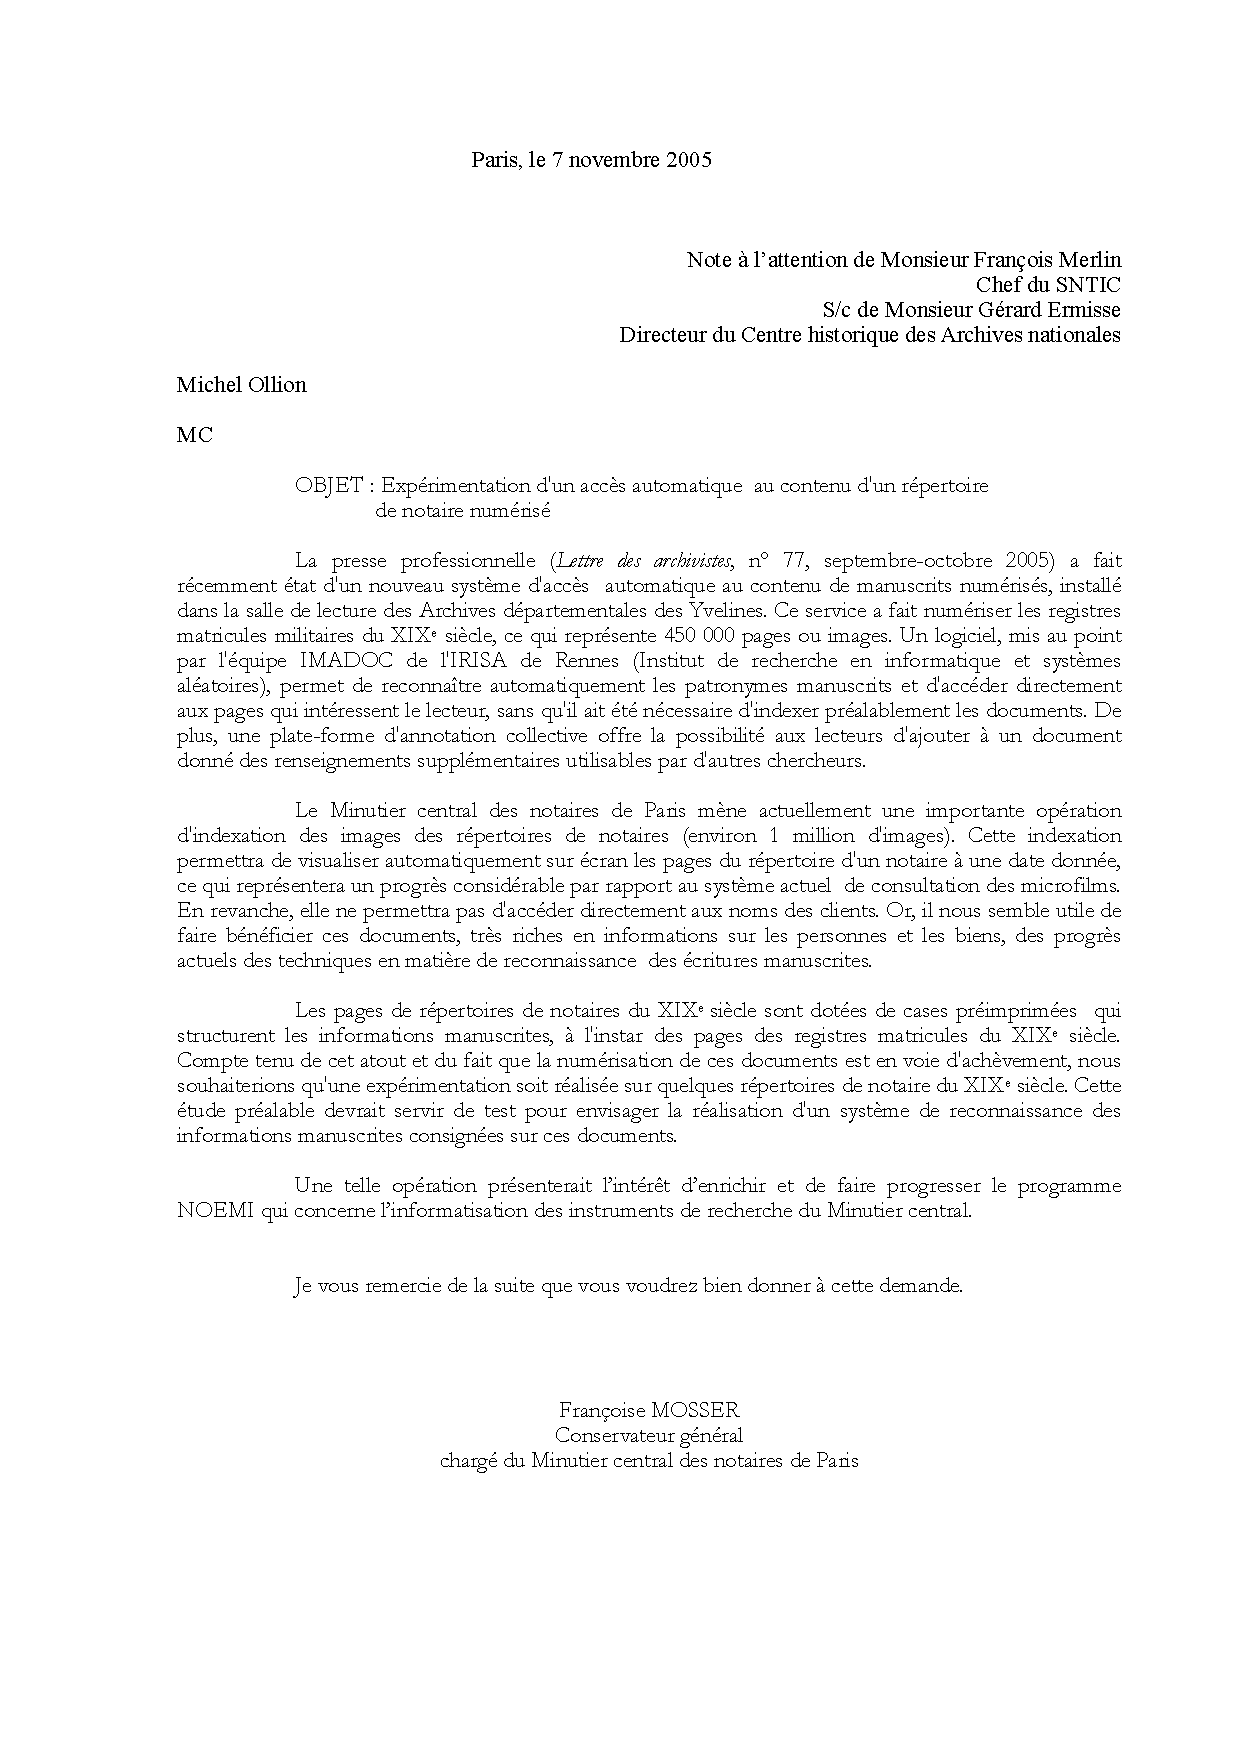
\includepdf{images_annexes/demande_ocr_Ollion.pdf}

\begin{figure}[h!]
    \centering
    \centerline{\fbox{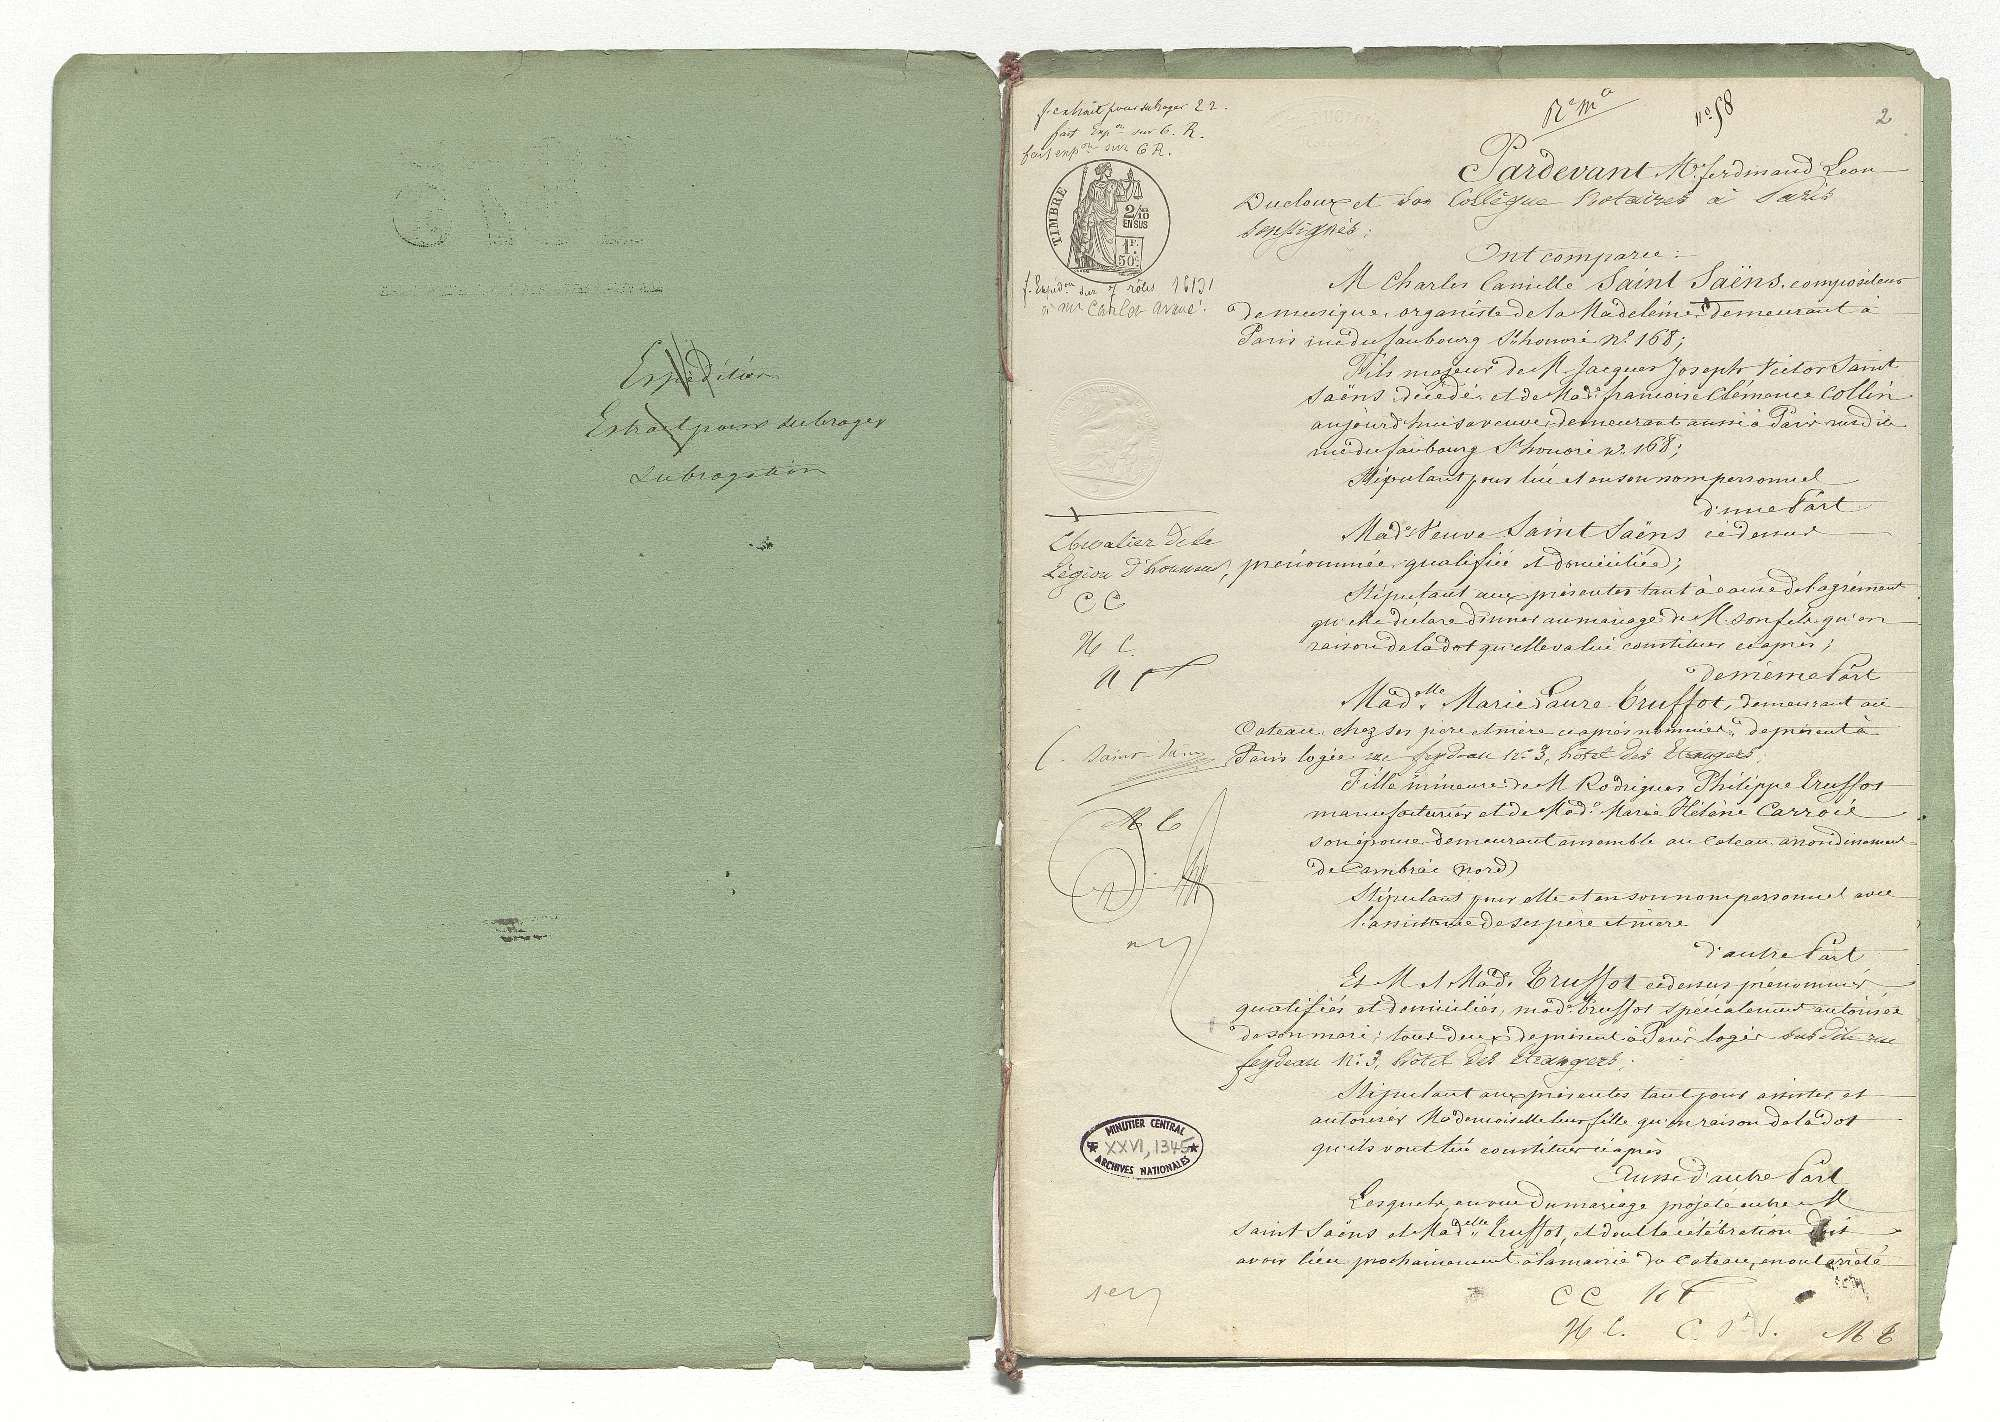
\includegraphics[width=19cm]{images_annexes/exemple_minute.jpg}}}
    \caption{Exemple de minute notariale \textcopyright Archives nationales/DMC, Minute \inquote{Contrat de mariage entre Charles Camille Saint-Saëns, compositeur de musique, organiste de la Madeleine demeurant au 168 rue du Faubourg Saint-Honoré, et Marie-Laure Truffot, fille de Rodrigue Truffot, manufacturier au Cateau-Cambrésis}, 18 janvier 1875,  MC/ET/XXVI/1345 (cote originale), MC/RS//872, lien vers la SIV : \url{https://www.siv.archives-nationales.culture.gouv.fr/siv/UD/FRAN_IR_041418/c1p6uqwjl1o3-xlv0cdl5wlgv}(consulté le 14/09/2020).}
    \label{fig:exemple_minute}
\end{figure}

\begin{figure}[h!]
    \centering
    \centerline{\fbox{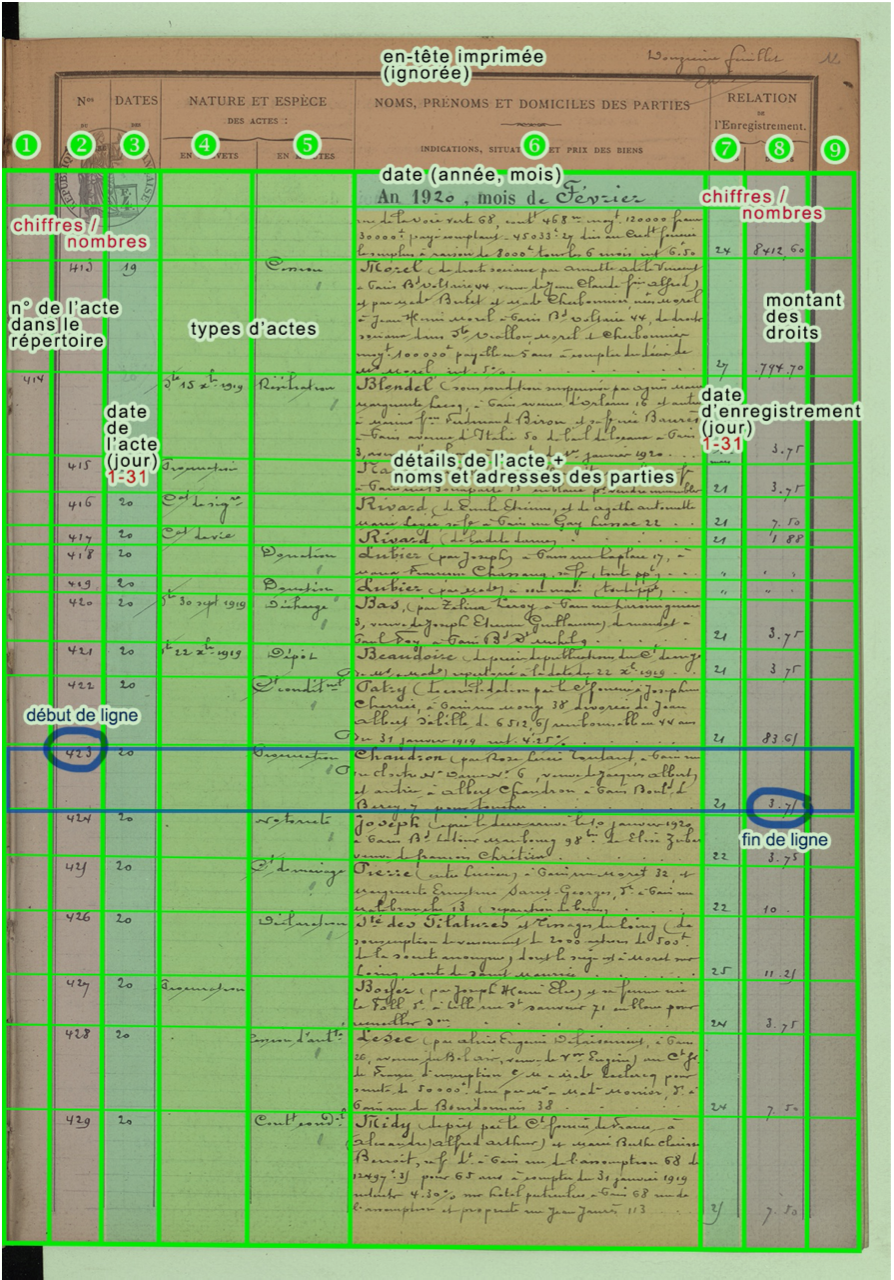
\includegraphics[width=14cm]{images_annexes/repertoire_structure_tableaux.png}}}
    \caption{Structuration en tableaux des répertoires \textcopyright \cite{bonhomme_defis_2018}, pp. 27.} 
    \label{fig:tableaux_repertoires}
\end{figure}

\begin{figure}[h]
    \centering
    \centerline{\fbox{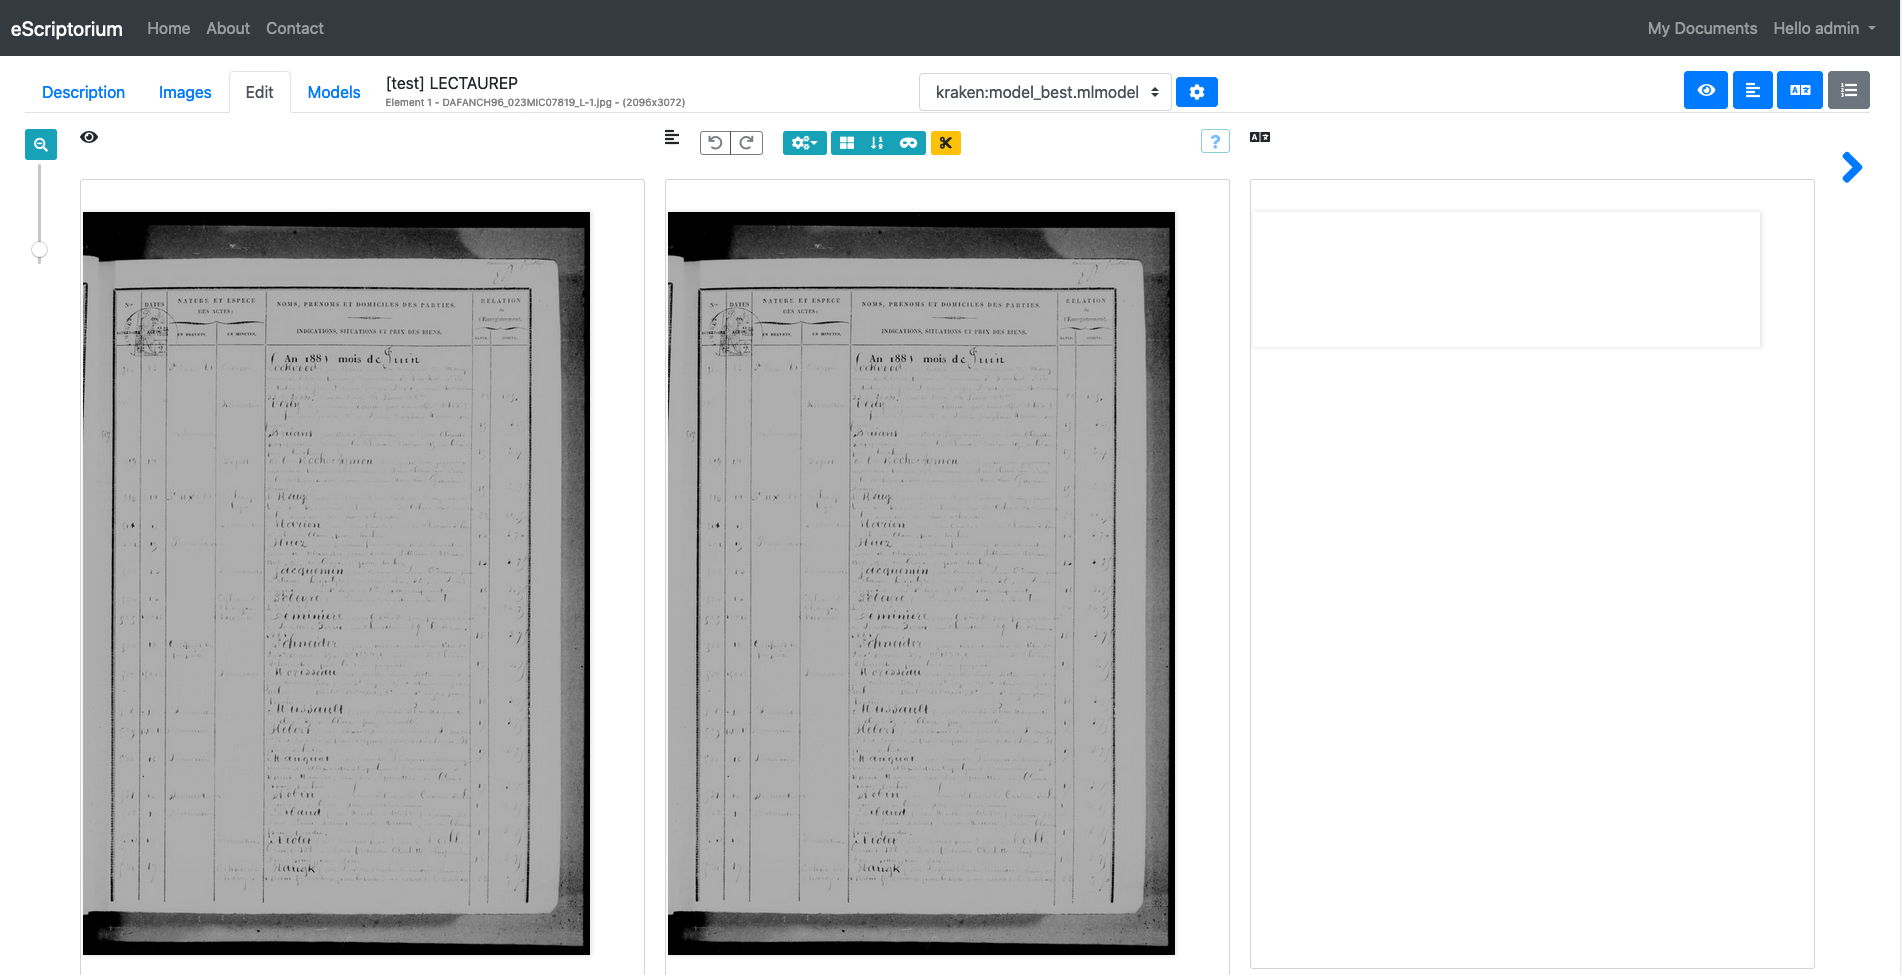
\includegraphics[width=18cm]{images_annexes/interface_eScriptorium.png}}}
    \caption{Application web eScriptorium \textcopyright L. Terriel, 2020, eScriptorium} 
    \label{fig:appli_eScriptorium}
\end{figure}

\begin{figure}[h]
    \centering
    \centerline{\fbox{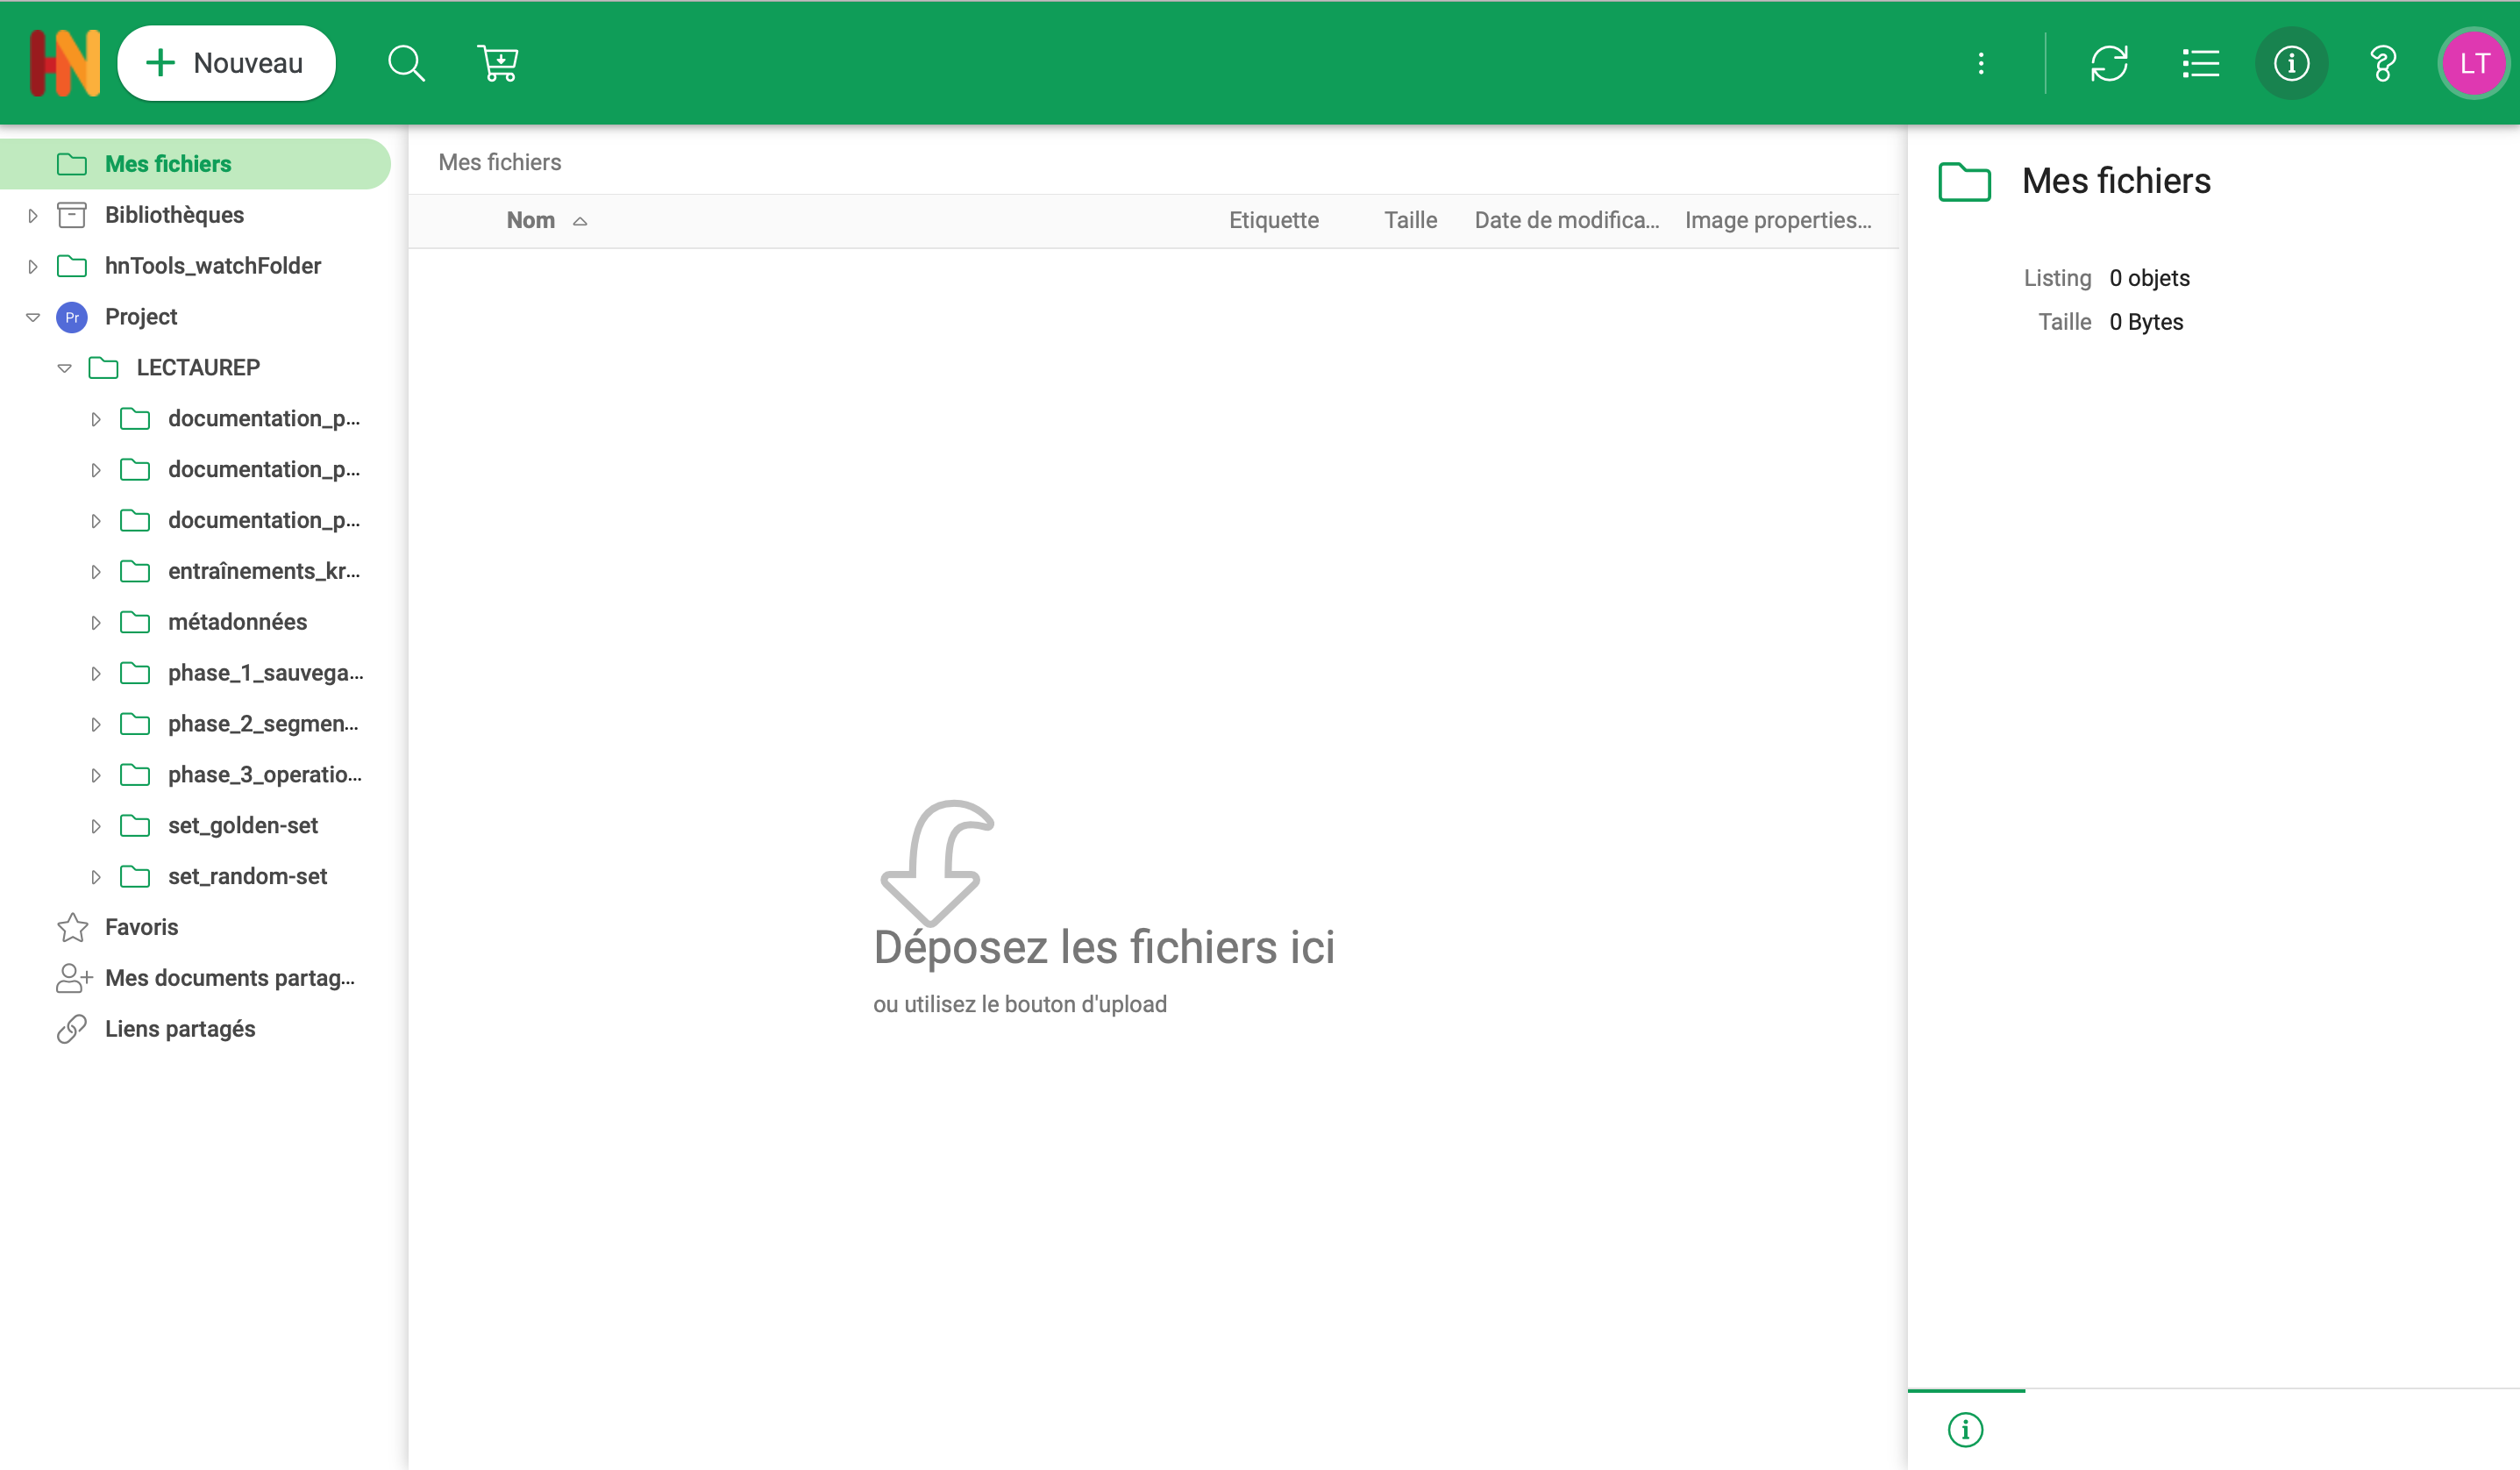
\includegraphics[width=18cm]{images_annexes/sharedocs.png}}}
    \caption{Exemple du \textit{Golden Set} et du \textit{Random Set} stockés sur \textit{Sharedocs} (Huma-num) \textcopyright L. Terriel, 2020, \textit{Sharedocs} (Huma-num)} 
    \label{fig:shareDocs}
\end{figure}

\begin{figure}[h!]
    \centering
    \centerline{\fbox{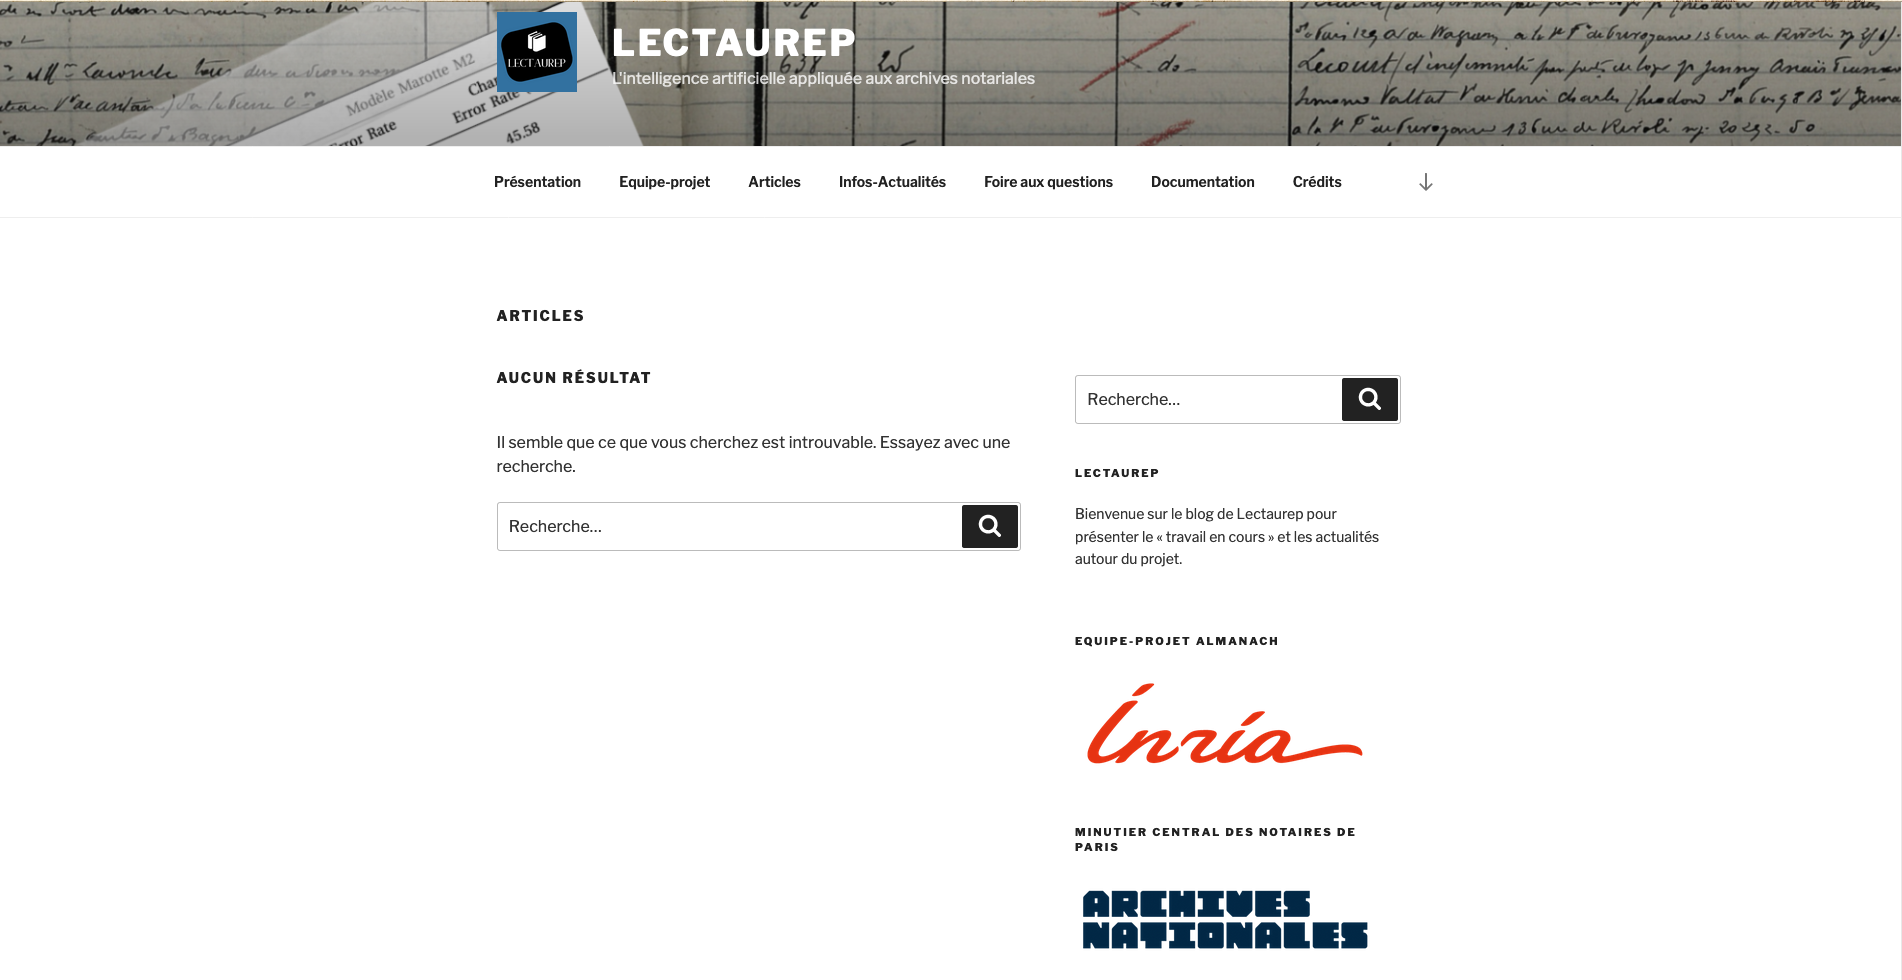
\includegraphics[width=18cm]{images_annexes/blog_lectaurep.png}}}
    \caption{Blog \textit{hypotheses.org} Lectaurep \textcopyright L. Terriel, blog \textit{hypotheses.org} Lectaurep}
    \label{fig:blog_lectaurep}
\end{figure}
\newpage
\thispagestyle{empty}
\chapter{Format pivot XML-TEI Lectaurep}\label{annexe_tei_pivot_prog}
localisation : \citecode{/B-Format\_pivot\_XML\_TEI\_Lectaurep} contenant :
\skip
\dirtree{%
.1 /B-Format\_pivot\_XML\_TEI\_Lectaurep/.
   .2 Doc/\DTcomment{regroupe la documentation sur le projet du fichier pivot XML TEI pour Lectaurep}.
        .3 Modélisation\_et\_documentation\_format\_pivot/.
           .4 template\_pivot\_TEI\_lectaurep.xml\DTcomment{Canevas (\textit{template}) pour formaliser les attentes et les réflexions des acteurs pour l'inclusion des données et des métadonnées Lectaurep dans le fichier pivot XML-TEI.}.
           .4 Les ODD aux formats : XML, PDF et HTML.\DTcomment{La documentation standard TEI pour le fichier pivot XML-TEI Lectaurep.}.
           .4 oddbyexample.xsl\DTcomment{Une feuille de transformation XSL pour générer une nouvelle ODD à partir de la \textit{template} XML-TEI pivot.}.
        .3 Crosswalks\_vers\_TEI\DTcomment{Un ensemble de transformations XSL utiles vers les spécifications TEI et ALTO, issues de différents projets.}.
            .4 ALTO -> TEI.
            .4 EAD -> TEI (2 versions).
            .4 ALTO -> TEI.
            .4 PAGE -> ALTO.
            .4 PAGE -> TEI.
   .2 Generator\_Lectaurep2TEI/\DTcomment{CLI Python permettant de simuler 
	                                     la conversion des données issues de Lectaurep (EAD-EAC, ALTO, EXIF) 
	                                     vers un fichier XML-TEI Pivot suivant les recommandations de l'ODD 
	                                     (voir le readme.md pour plus de détails).}.
        .3 Output/\DTcomment{Dossier dans lequel est généré la sortie du script.}.
            .4  test\_legay\_tei.xml\DTcomment{Exemple de fichier pivot TEI Lectaurep de test généré en sortie du script.}.
        .3 Sets\_test\_Legay/\DTcomment{Contient un ensemble de fichiers correspondant aux données fournies par Lectaurep pour tester le programme \textit{generator Lectaurep2TEI} et généré une première version du format pivot.}.
            .4  Data\_xml\_alto/\DTcomment{fichiers XML ALTO correspondants aux transcriptions vérité terrain récupérés sur l'espace \textit{ShareDocs} relatives aux images numérisées du répertoire de notaire d'Ernest Legay (étude XXIII).}.
            .4  Data\_xml\_ead\_eac/\DTcomment{fichiers XML EAD et XML EAC-CPF correpondants aux instruments de recherche des répertoires du notaire Ernest Legay (étude XXIII) et notices producteurs récupérées sur la Salle des inventaires virtuels des Archives nationales.}.
                .5 FRAN\_IR\_041698.xml \DTcomment{IR \inquote{Minutes et répertoires du notaire Ernest LEGAY, 25 février 1875 - 14 mai 1902 (étude XXIII)}.}.
                .5 FRAN\_IR\_051379.xml \DTcomment{IR \inquote{Images des répertoires du notaire Ernest Legay pour l'étude XXIII}.}.
                .5 FRAN\_NP\_010150.xml \DTcomment{Notice producteur de l'étude XXIII.}.
                .5 FRAN\_NP\_010150.xml \DTcomment{Notice producteur de Legay, Ernest.}.
                .5 Schémas XML et DTD EAD et EAC-CPF.
            .4  images/\DTcomment{Images numérisées du répertoire de notaire d'Ernest Legay (étude XXIII) issues du \textit{Golden Set} de l'espace \textit{ShareDocs}.}.
        .3 generator\_utils/.\DTcomment{Ensemble des modules Python utiles au fonctionnement du CLI \textit{generator Lectaurep2TEI}. Pour les détails des fonctions consulter les \textit{docstrings} dans les scripts.}.
            .4  \_\_init\_\_.py.
            .4  build\_utils.py.
            .4  extract\_utils.py.
            .4  validation\_utils.py.
        .3 pack\_schemaRNG/.\DTcomment{Doit accueillir à terme les schémas de validation Relax NG du fichier pivot XML-TEI Lectaurep.}.
            .4 tei\_all.rng.\DTcomment{Schéma Relax NG \textit{TEI ALL}.}.
        .3 Lectaurep\_ALTO2TEI.xsl.\DTcomment{Une feuille de transformation XSL ALTO vers TEI nécessaire pour le fonctionnement du script principal. Pour plus de détails consulter la \textit{docstring} de la feuille.}.
        .3 Lectaurep\_EADEAC2TEI.xsl.\DTcomment{Une feuille de transformation XSL EAD/EAC vers TEI nécessaire pour le fonctionnement du script principal. Pour les usages consulter la \textit{docstring}.}.
        .3 catalog\_alto.xml.\DTcomment{Fichier automatiquement créé par le script, nécessaire pou l'usage de la fonction Xpath 2.0 \citecode{collection()} pour la feuille XSL \citecode{Lectaurep\_ALTO2TEI.xsl}}.
        .3 catalog\_ead\_eac.xml.Lectaurep\_ALTO2TEI.xsl\DTcomment{Fichier automatiquement créé par le script, nécessaire pou l'usage de la fonction Xpath 2.0 \citecode{collection()} pour la feuille XSL \citecode{Lectaurep\_EADEAC2TEI.xsl}}.
        .3 generator\_Lectaurep2TEI\_logo.png.
        .3 inr\_logo\_grisbleu.png.
        .3 main.py.\DTcomment{Script Python principal d'exécution du CLI \textit{generator Leactaurep2TEI}.}.
        .3 readme.md.\DTcomment{Documentation pour installer et lancer le programme.}.
        .3 requirements.txt.\DTcomment{Ensemble des \textit{packages} Python nécessaires à l'utilisation du CLI}.
        .3 snap\_generator.png.
        }
\newpage
\thispagestyle{empty}
\chapter{Application \textit{Kraken Benchmark}}\label{annexe_KB}
localisation : \citecode{/C-Application\_Kraken\_Benchmark} contenant :
\skip
\dirtree{%
.1 /C-Application\_Kraken\_Benchmark/.
   .2 Documentation-Reasearch/.\DTcomment{Contient les versions du \textit{notebook Jupyter} exposant les réflexions sur les métriques et les algorithmes utilisés dans l'application \textit{Kraken-Benchmark}.}.
    .3 Evaluation de la similarité entre deux séquences dans le contexte de la reconnaissance automatique de caractères.\DTcomment{\textit{notebook} Jupyter en versions PDF, HTML et IPYNB (format natif).}. 
    .3 Ensemble d'images rattachés au \textit{notebook} Jupyter.
   .2 KB-app/.\DTcomment{Dossier contenant les fichiers pour faire fonctionner l'application \textit{\textit{Kraken-Benchmark}}.}.
    .3 STS\_Tools/.\DTcomment{Le \textit{package} Python \textit{Sequences to Similarity} créée pour l'application \textit{\textit{Kraken-Benchmark}} contient deux modules Python.}.
        .4 STSig.py.\DTcomment{module Python \textit{Sequences To Signals} (en cours de développement); module pour créer des visualisations et des métriques expérimentales pour comparer deux chaînes de caractères.}.
        .4 SynSemTS.py.\DTcomment{module Python \textit{Syntactic Semantic To Similarity} qui contient la plupart des métriques (syntaxiques et sémantiques) et les visualisations associées; utilisé dans l'application pour l'analyse de deux chaînes de caractères correspondant à la vérité terrain et la transcription issue du système HTR.}.
        .4  \_\_init\_\_.py.
    .3 kb\_report/.\DTcomment{Dossier contenant les fichiers pour la gestion de la partie affichage dans le navigateur de l'application via le \textit{package} \textit{Flask}.}.
        .4  static/.\DTcomment{contient les images de l'application à afficher dans le navigateur.}.
        .4  templates/.\DTcomment{contient les pages HTML de l'application.}.
        .4  \_\_init\_\_.py.
        .4  routing.py\DTcomment{Script Python qui contient les différentes routes URL de l'application.}.
    .3 kb\_utils/.\DTcomment{Dossier contenant un module Python nécessaire au fonctionnement de l'application.}.
        .4  \_\_init\_\_.py.
        .4  kb\_utils.py.\DTcomment{Module Python contenant des fonctions utiles au fonctionnement de l'application.}.
    .3 environment.yml.\DTcomment{Fichier pour la création d'un environnement virtuel \textit{Conda} contenant les \textit{packages} Python nécessaires.}.
    .3 kraken\_benchmark.py.\DTcomment{Script principal pour l'exécution de l'application \textit{Kraken-Benchmark}.}.
   .2 sets\_test/.\DTcomment{Jeux de fichiers pour effectuer des tests dans \textit{Kraken-Benchmark} et scripts Python complémentaires.}.
    .3 jules\_verne\_set\_test/.\DTcomment{Jeux de données utilisés pour les tests fonctionnels de l'application.}.
        .4  images/.\DTcomment{Contient des numérisations (formats \citecode{.jpeg}) de l'ouvrage \textit{Voyage au centre de la terre} récupérés sur \og Gallica\fg{}}.
        .4  dataset\_GT/.\DTcomment{Contient les vérités terrains en format texte brut utilisées pour comparer les résultats issus de l'HTR de \textit{Kraken-Benchmark}. Édités à partir du CLI Kraken.}.
        .4  model/.\DTcomment{Contient le modèle (format \citecode{.mlmodel}) entraîné sur le CLI Kraken pour réaliser l'OCR dans \textit{Kraken-Benchmark} sur le \textit{set} de numérisations de \textit{Voyage au centre de la terre}.}.
    .3 sets\_tests\_lectaurep/.\DTcomment{Jeux de données utilisés pour tester les modèles de transcription issus du CLI Kraken sur des images de répertoires de notaires sélectionnés pour leurs particularismes (pour plus de détails sur les sets d'images et les modèles HTR utilisés voir le fichier \citecode{CR\_tests\_lectaurep\_KB.md}) pour évaluer la qualité des transcriptions. pour plus de précisions, Cf. section \ref{tests_KB_lectaurep}}.
        .4  different\_control\_set/.\DTcomment{Contient les transcriptions vérité terrains (\citecode{GT} et les images).}.
        .4  homogeneous\_control\_set/.\DTcomment{Contient les transcriptions vérité terrains (\citecode{GT} et les images).}.
        .4  set\_material\_defects/.\DTcomment{Contient les transcriptions vérité terrains (\citecode{GT} et les images).}.
        .4  set\_writing\_defects/.\DTcomment{Contient les transcriptions vérité terrains (\citecode{GT} et les images).}.
        .4  snaps\_tests\_lectaurep/.\DTcomment{Contient des sauvegardes des pages HTML de l'application \textit{Kraken-Benchmark} réalisés lors des différents tests Lectaurep.}.
            .5 report\_html/.\DTcomment{Contient des captures de la page d'accueil de \textit{Kraken-Benchmark} avec les principales métriques.}.
            .5 versus\_text\_html/.\DTcomment{Contient des captures de la fonctionnalité \textit{versus text} (comparaison de la vérité terrain et de la transcription HTR dans \textit{Kraken-Benchmark}).}.
        .4  models/.\DTcomment{Contient les modèles HTR, entraînés avec le CLI \textit{Kraken}, et utilisés sur les différents jeux de données.}.
        .4  CR\_tests\_lectaurep\_KB.md\DTcomment{Compte-rendu présentant le déroulement des tests, la description des sets de tests, des modèles et des résultats des expériences.}.
        .4  details\_data\_average\_tests\_model\_test\_lectaurep\_bin\_accuracy\_6064.mlmodel - Feuille 1.pdf\DTcomment{Fichier PDF présentant la moyenne des résultats des tests avec le modèle 6064, utilisé pour le graphique radar.}.
        .4   details\_data\_average\_tests\_model\_test\_lectaurep\_bin\_accuracy\_8164.mlmodel - Feuille 1.pdf\DTcomment{Fichier PDF présentant la moyenne des résultats des tests avec le modèle 8164, utilisé pour le graphique radar.}.
        .4  radar\_test\_II\_model\_0-8164.png\DTcomment{Graphique du model 8164.}.
        .4  radar\_test\_I\_model\_0-6064.png\DTcomment{Graphique du model 6064.}.
    .3 alto2text.py.\DTcomment{Script Python adapté, provenant de la \textit{StaatsbibliothekBerlin} permettant la conversion de certaines transcriptions vérités terrains en XML ALTO vers des fichiers texte brut.}.
    .3 radar\_graph.py.\DTcomment{Script Python adapté permettant la génération d'un graphique radar, utile pour le rapport concernant les tests spécifiques à Lectaurep durant le stage.}.
   .2 README.md.\DTcomment{Présentation et documentation principale de l'application pour l'installation et l'utilisation de \textit{Kraken-Benshmark}.}.
   .2 ci-test.sh.\DTcomment{Script Bash (Alix Chagué) pour configurer les tests de l'application (avec le logiciel \citecode{Pylint}) doit accueillir l'appel des tests unitaires.}.
   .2 .pylintrc.\DTcomment{fichier pour configurer \citecode{Pylint}.}.
   .2 requirements.txt.\DTcomment{fichiers utilisés exclusivement par le script \citecode{ci-test.sh}.}.
   }
\newpage
\thispagestyle{empty}
\chapter{Documents de travail pour le fichier pivot XML-TEI Lectaurep}\label{doc_ax_tei_pivot}
localisation : \citecode{/D-Doc\_travail\_pivot\_tei\_lectaurep} contenant :

\begin{itemize}
    \item \citecode{modèle\_metadonnées\_vise\_V4.png} ou Figure \ref{fig:modele_vise_V4}
    \item \citecode{Generateur-XML-TEI.png} ou Figure \ref{fig:generateur_tei}
\end{itemize}

% Figures en dessous : 

\begin{figure}
  \begin{sideways}
    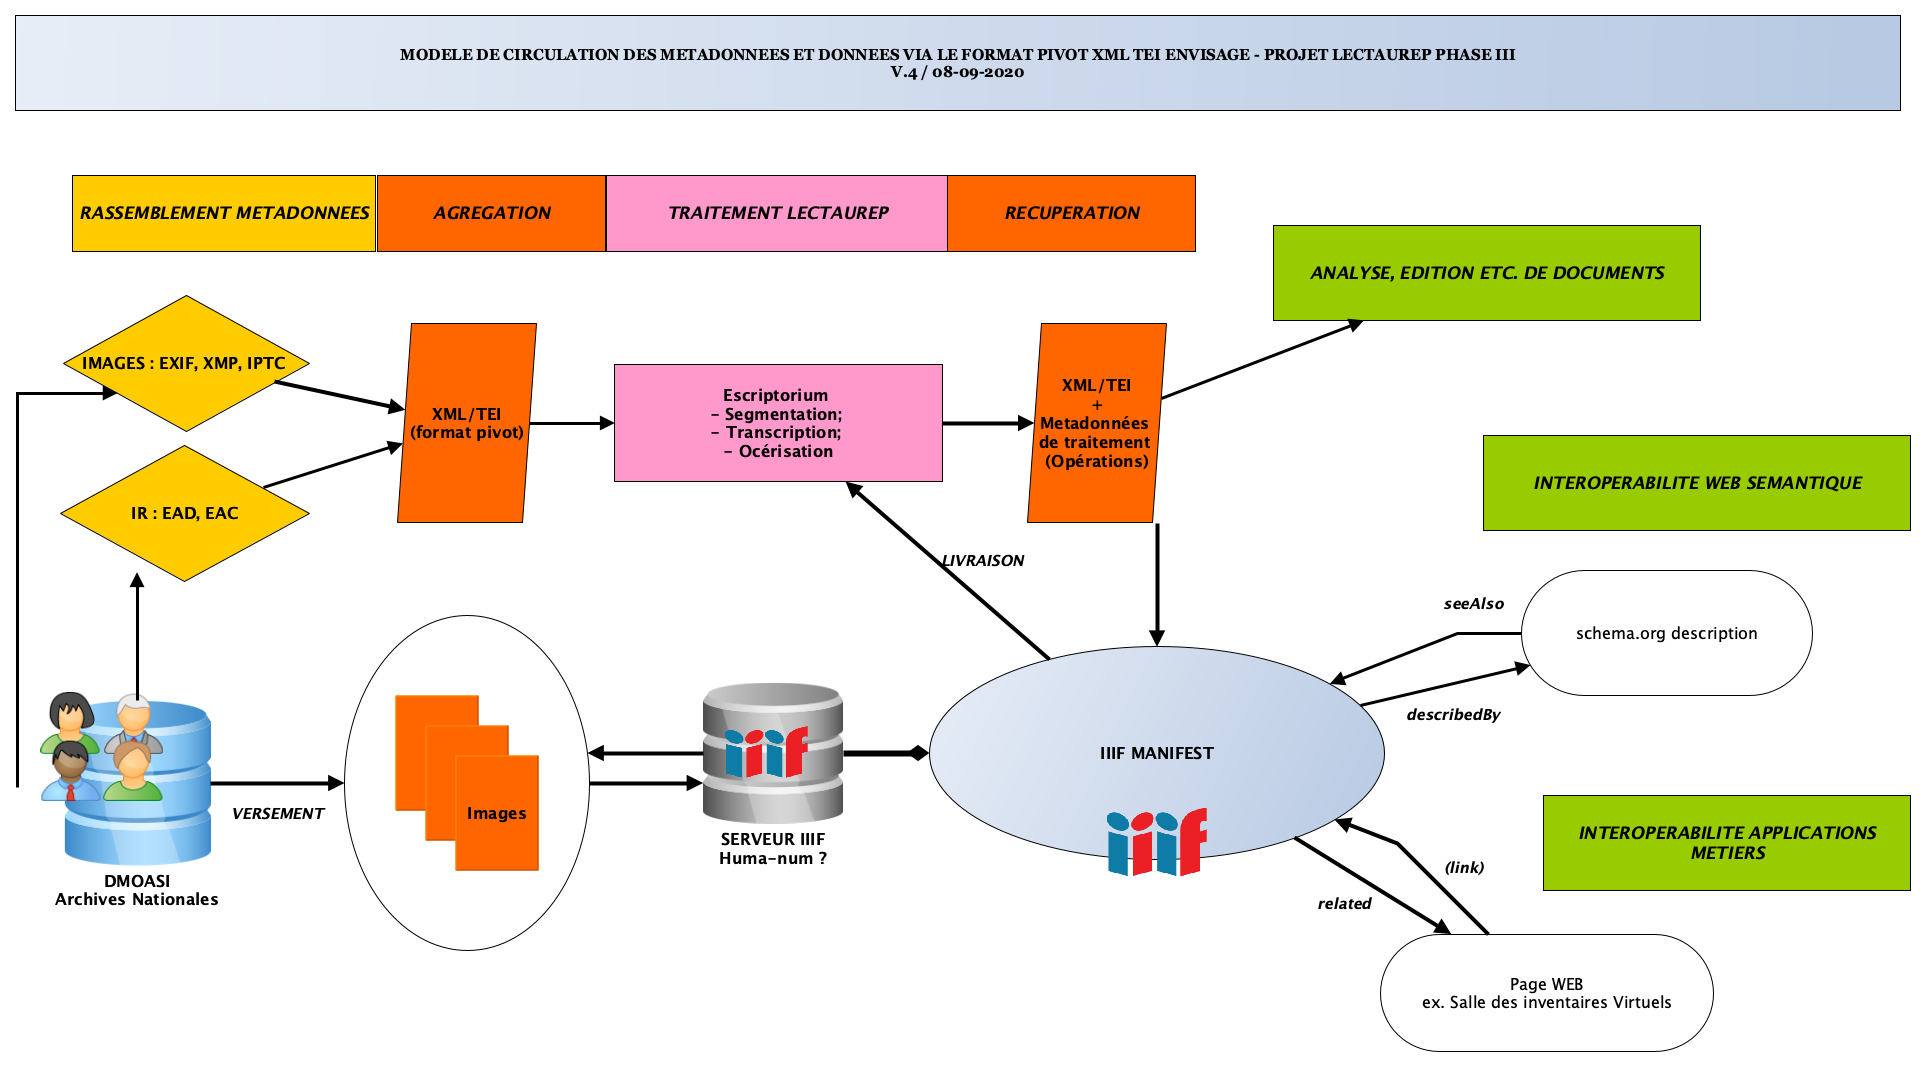
\includegraphics[width=24cm, height=16cm]{images_annexes/modèle_metadonnées_vise_V4.png}
  \end{sideways}
  \centering
  \caption{Schématisation du modèle de circulation des données dans eScriptorium souhaité par Lectaurep à terme  \textcopyright L. Terriel, 2020, yEd}
  \label{fig:modele_vise_V4}
\end{figure}

\begin{figure}
    \centering
    \centerline{\fbox{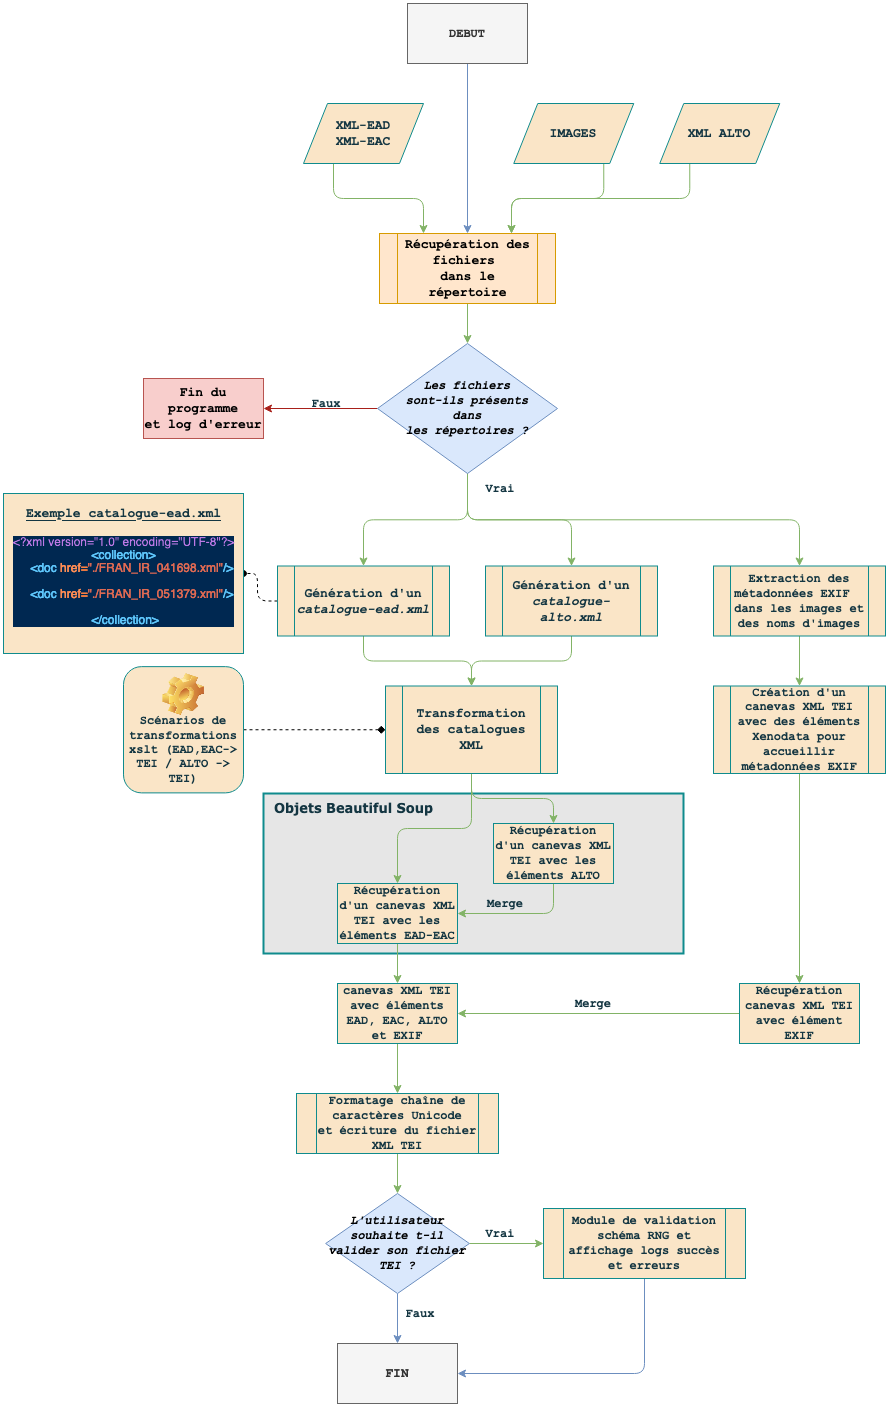
\includegraphics[width=18cm, height=22.5cm]{images_annexes/Generateur-XML-TEI.png}}}
    \caption{Algorigramme du programme Generator Lectaurep-TEI pour simuler la visualisation d'un format XML TEI pivot comprenant des données provenant de fichiers XML ALTO, EAD et EAC-CPF et des métadonnées EXIF provenant d'images.   \textcopyright L. Terriel, 2020, Diagrams.net}
    \label{fig:generateur_tei}
\end{figure}

\chapter{Documents de travail pour \textit{\textit{Kraken-Benchmark}}}\label{doc_ax_kb}
localisation : \citecode{/E-Doc\_travail\_KB} contenant :

\begin{itemize}
    \item \citecode{detail-model-transkribus.png} ou Figure \ref{fig:details-model-transkribus}
    \item \citecode{compare-texts-transkribus.png} ou Figure \ref{fig:compare-texts-transkribus}
    \item \citecode{Kraken-Benchmark\_modelisation.png} ou Figure \ref{fig:algo-kb}
\end{itemize}

% Figures en dessous :
\begin{figure}
    \centering
    \centerline{\fbox{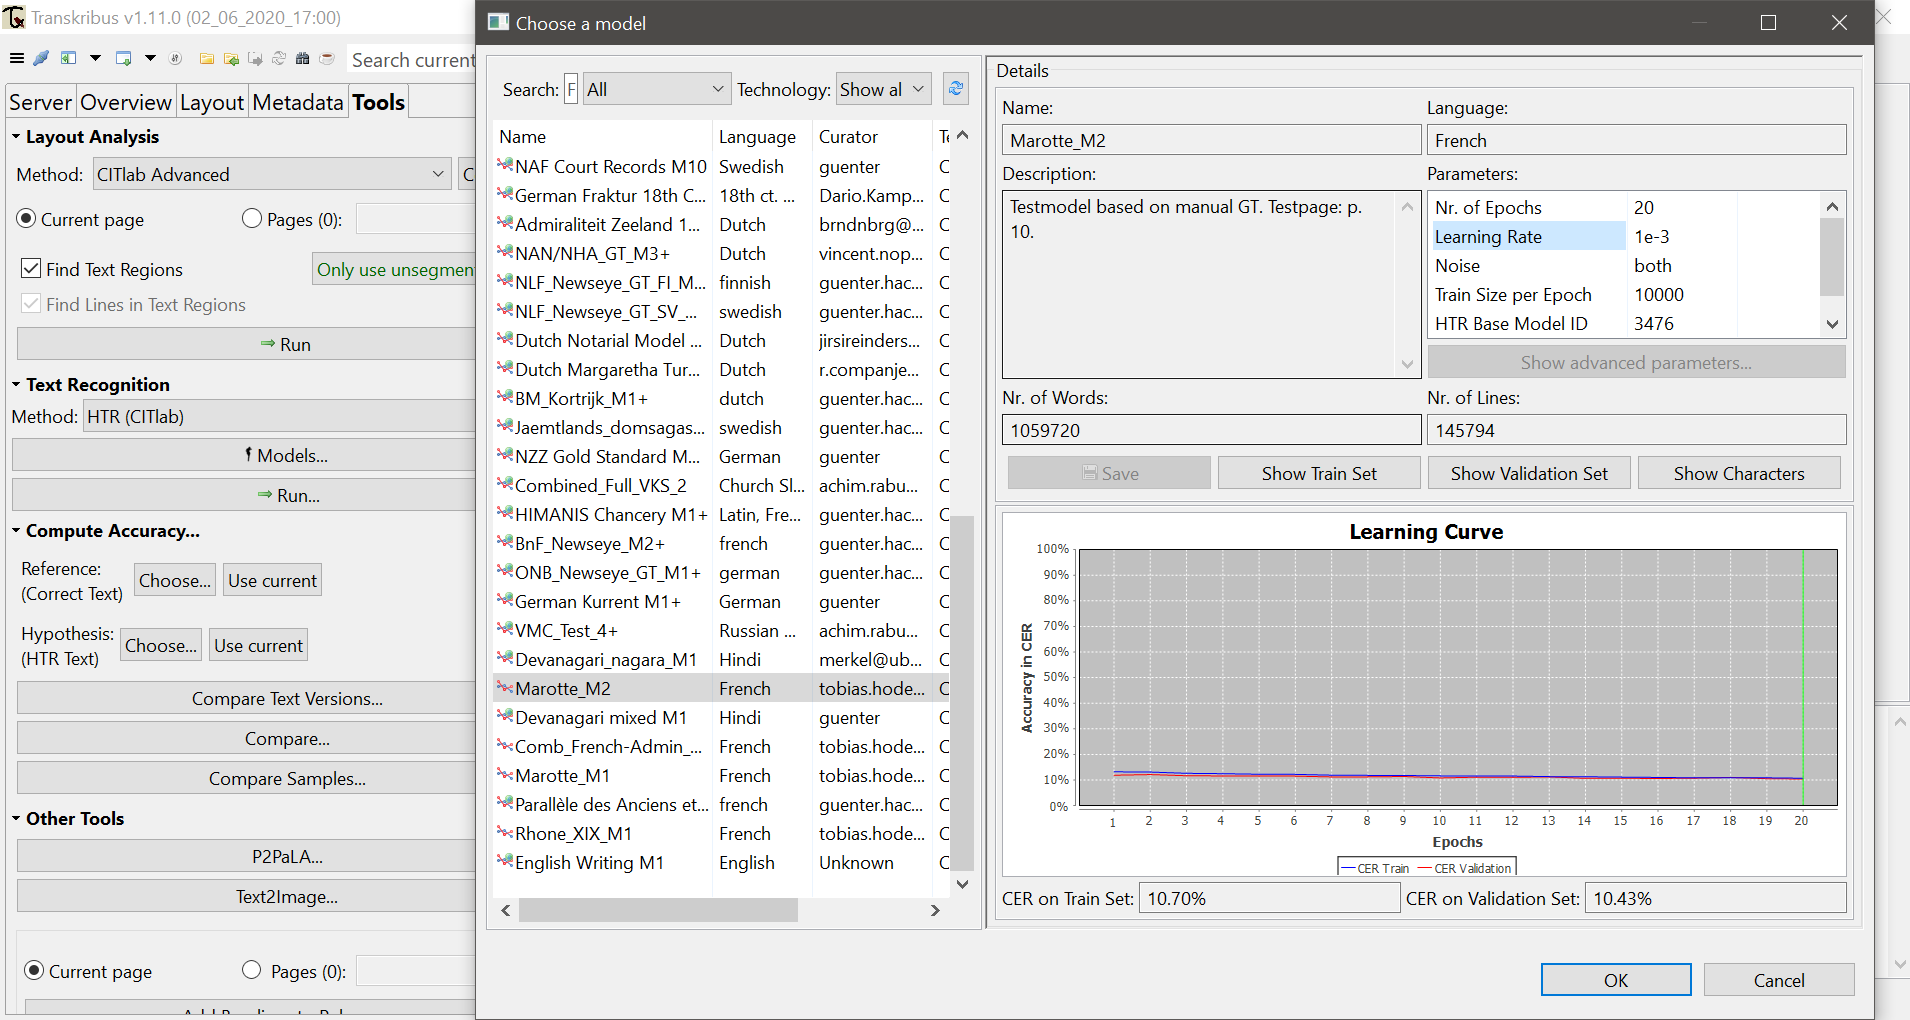
\includegraphics[width=18cm]{images_annexes/detail-model-transkribus.png}}}
    \caption{fenêtre pour visualiser des détails concernant le modèle envoyé dans l'interface \textit{Transkribus} \textcopyright A. Chague, 2020, \textit{Transkribus}}
    \label{fig:details-model-transkribus}
\end{figure}

\begin{figure}
    \centering
    \centerline{\fbox{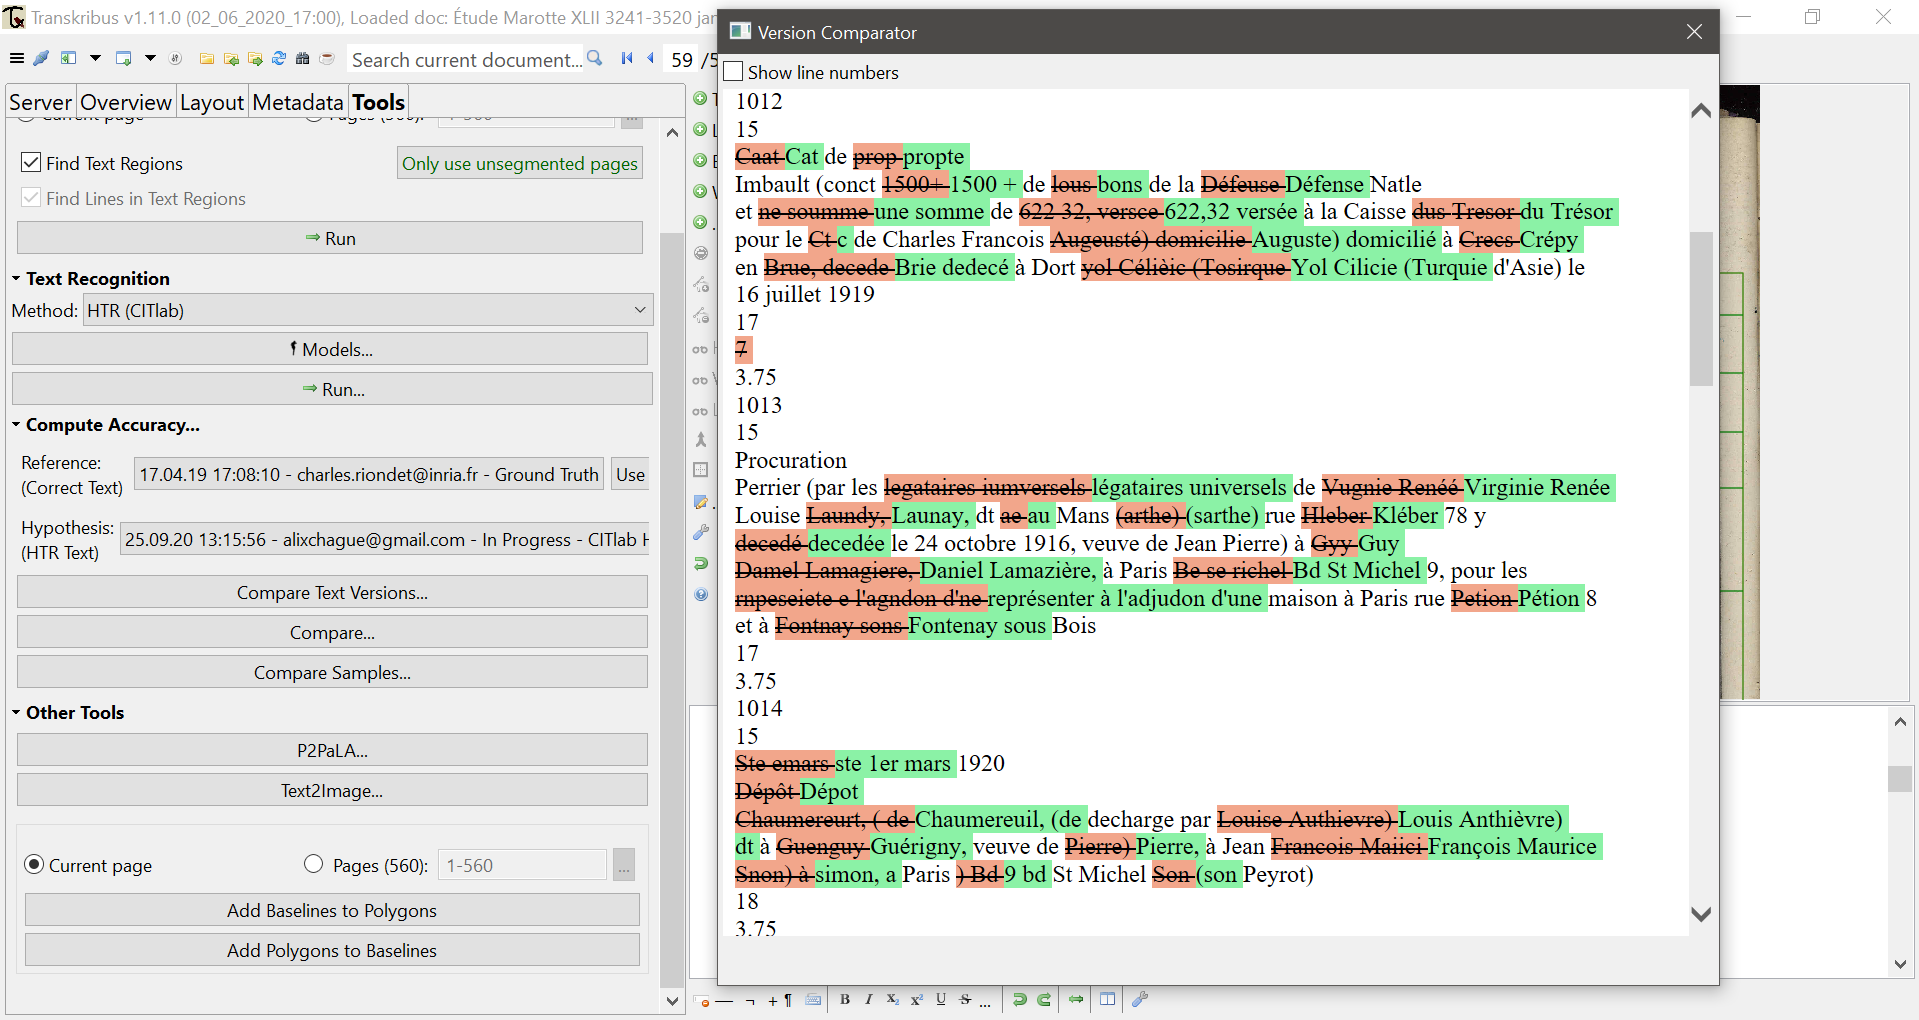
\includegraphics[width=18cm]{images_annexes/compare-texts-transkribus.png}}}
    \caption{fenêtre pour comparer la référence et la prédiction dans l'interface \textit{Transkribus} \textcopyright A. Chague, 2020, \textit{Transkribus}}
    \label{fig:compare-texts-transkribus}
\end{figure}

\begin{figure}
    \centering
    \centerline{\fbox{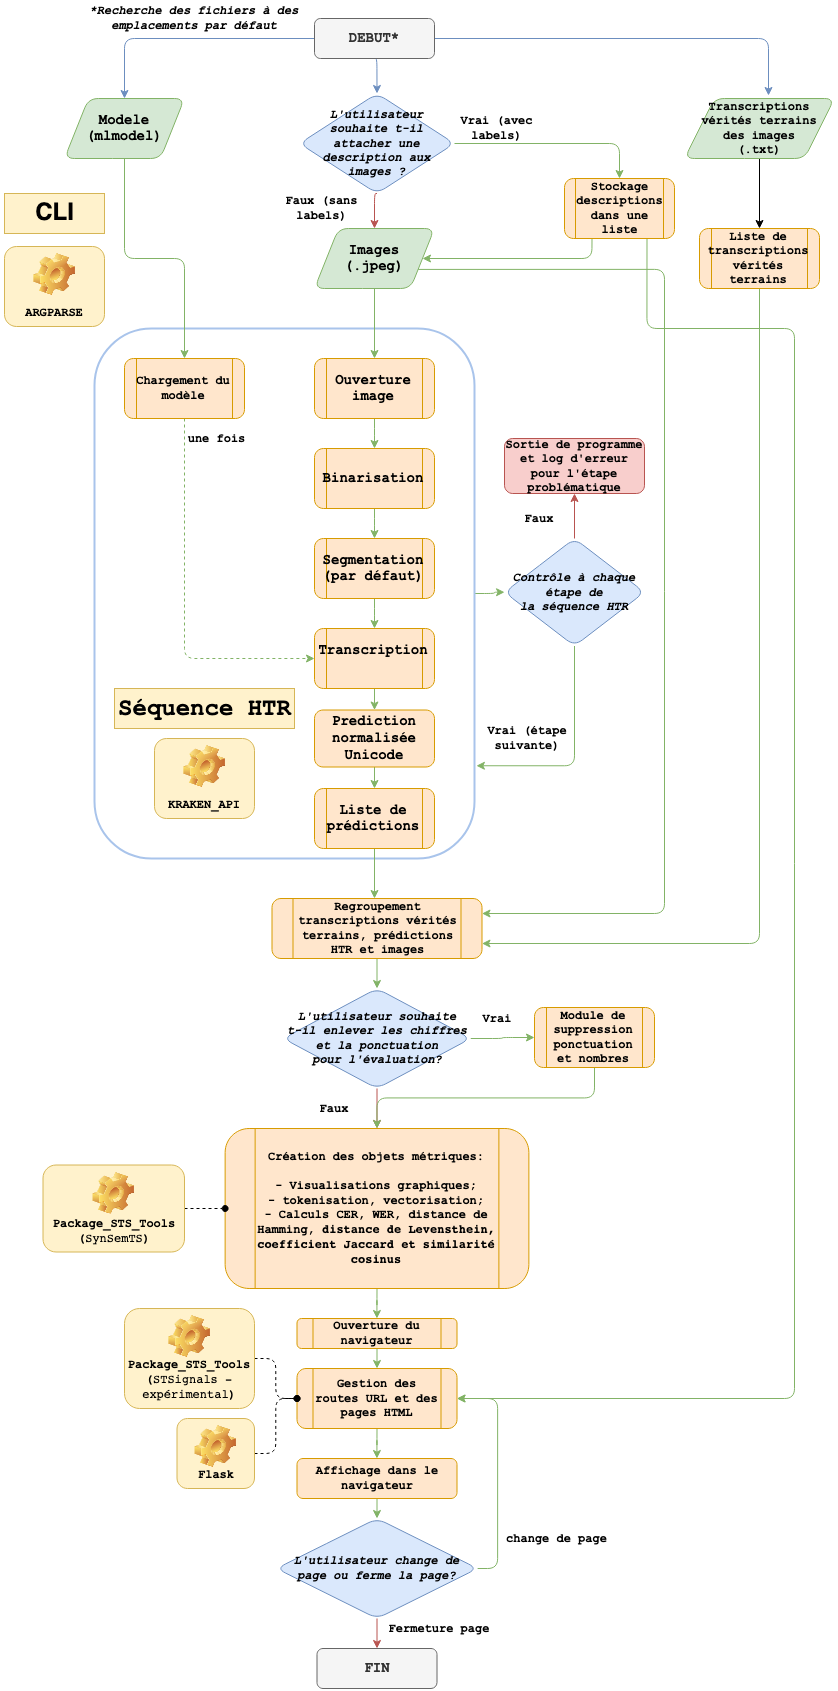
\includegraphics[width=18cm, height=22.5cm]{images_annexes/Kraken-Benchmark_modelisation.png}}}
    \caption{Algorigramme de Kraken-Benchmark.   \textcopyright L. Terriel, 2020, Diagrams.net}
    \label{fig:algo-kb}
\end{figure}

\chapter{Scripts Python complémentaires}
localisation : \citecode{/F-scripts\_python} contenant :

\begin{itemize}
    \item \citecode{script\_python\_POS.py} ou Figure \ref{fig:script_python_POS}
    \item \citecode{script\_python\_exif.py} ou Figure \ref{fig:script_python_exif}
    \item \citecode{script\_calc\_RO.py} ou Figure \ref{fig:script_calc_RO}
\end{itemize}

\begin{figure}[h]
\lstset{language=Python}
\begin{lstlisting}
"""
Exemple de script pour l'étiquetage morpho-syntaxique (part-of-speech)

Auteur : Lucas Terriel
Date : 14/09/2020
"""

# On importe le package spacy (tâches NLP)
import spacy
from spacy import displacy

# On charge un modèle français
# ! préalable télécharger le modèle (réseau convolutionnel entraîné sur deux corpus, WikiNER et Sequoia) !
# python -m spacy download fr_core_news_sm
model_fr = spacy.load("fr_core_news_sm")

# On défini une phrase de test
test = "Dussuel (par Paul Charles Claude) demeurant à Paris"

def return_POS(sentence):
    """
    fonction pour tokeniser la phrase et retourner les étiquettes grammaticale
    de chaque token.

    :param sentence: phrase
    :type sentence: str
    :return: token et étiquettes POS
    :type return : list
    """
    # Découpage de la phrase en mots (tokens)
    document = model_fr(sentence)
    # Retourne dans un dictionnaire les tokens (X) -clés- et leurs étiquettes (X.pos_) -valeurs- à partir d'une liste en compréhension
    return [{(X, X.pos_)} for X in document]

# affichage du dictionnaire
print(return_POS(test))

# Pour la visualisation dans le navigateur du POS on défini des paramètres de style
options = {"color": "red", "font": "Source Sans Pro"}

# Visualisation POS dans le navigateur
doc = model_fr(test)
displacy.serve(doc, style="dep", options=options)

\end{lstlisting}
\caption{Script Python pour effectuer de l'étiquetage morpho-syntaxique (POS) \textcopyright L. Terriel, 2020}
\label{fig:script_python_POS}
\end{figure}

\begin{figure}[h]
\lstset{language=Python}
\begin{lstlisting}
"""
Exemple de script pour afficher les métadonnées EXIF d'une image

Auteur : Lucas Terriel
Date : 14/09/2020
"""

# import du module pyExifTool pour l'extraction de métadonnées Exif
import exiftool

# Création de l'objet ExifTool, on localise l'image et récupération des métadonnées dans un dictionnaire (possibilité de traiter en lot - batch)
with exiftool.ExifTool() as et:
    metadata = et.get_metadata('../static/Voyage_au_centre_de_la_
    [...]Verne_Jules_btv1b8600259v_16.jpeg')

# Affichage des métadonnées à partir du dictionnaire
for key, value in metadata.items():
    print(f'{key} => {value}')

\end{lstlisting}
\caption{Script Python pour afficher les métadonnées Exif d'une image \textcopyright L. Terriel, 2020}
\label{fig:script_python_exif}
\end{figure}

\begin{figure}[h]
\lstset{language=Python}
\begin{lstlisting}
"""
Script pour afficher un score de similarité basé sur l'algorithme Ratcliff/Obershelp

Auteur : Lucas Terriel
Date : 14/09/2020
"""

# On importe le module built-in implémentant l'algorithme Ratcliff/Obershelp
import difflib

# On récupère le score 
similarite_ro = difflib.SequenceMatcher(None, "En l'an 1920 par la procuration", "En l'an 1920 par le procureur").ratio()

# On affiche le score
print(f'Le score de similarité est de : {similarite_ro}')

>>> Le score de similarité est de : 0.8333333333333334

\end{lstlisting}
\caption{Script Python pour calculer un score de similarité suivant l'algorithme Ratcliff/Obershelp  \textcopyright L. Terriel, 2020}
\label{fig:script_calc_RO}
\end{figure}

\part*{Bibliographie}
\addcontentsline{toc}{part}{Bibliographie}
\markboth{Bibliographie}{Bibliographie}
\nocite{*}

\printbibliography[keyword={hist\_not},title={Histoire quantitative et notariale}]
\printbibliography[keyword={XIX},title={Ressources sur les écritures XIX$^{e}$ siècle}]
\printbibliography[keyword={archivistique},title={Archivistique}]
\printbibliography[keyword={hum\_num},title={Humanités numériques}]
\printbibliography[keyword={pp},title={Projets patrimoniaux et numérique}]
\printbibliography[keyword={Données \& analyses},title={Données et analyses}]
\printbibliography[keyword={ia},title={IA, TAL et HTR}]
\printbibliography[keyword={xml},title={Langage XML et standards}]
\printbibliography[keyword={logiciels},title={Logiciels et services}]
\printbibliography[keyword={package},title={Documentation \textit{packages} Python}]
\printbibliography[keyword={utilitaires},title={Utilitaires}]
\backmatter
\chapter*{Lexique des termes informatiques}
\addcontentsline{toc}{chapter}{Lexique des termes informatiques}
\markboth{Lexique des termes informatiques}{} 

\textit{\small{Liste non exhaustive}}

\begin{itemize}
    \item \textbf{Algorithme} : Suite d'étapes réalisées par un programme informatique pour effectuer une tâche.
    \item \textbf{\textit{Back-office/Front-office}} : Dans une application, désigne la partie visible par le client (\textit{front-office}) et la partie qui concerne les systèmes d'informations (bases de données) et leur gestion, invisible pour l'utilisateur final (\textit{back-office}).
    \item \textbf{\textit{Blog}} : Type de site \textit{web} qui permet la publication périodique d'articles scientifiques rendant compte de l'actualité d'un projet ou d'une thématique.
    \item \textbf{Interface en ligne de commande} : CLI ou \textit{Command Line Interface} en anglais - interface homme machine dépourvue d'aspect graphique et où la communication s'effectue en mode texte, au moyen de lignes de commande (texte entré à l'aide du clavier) pour demander à l'ordinateur d'effectuer une opération.
    \item \textbf{\textit{Commit}} : Dans un système de versionnage, commande qui permet de valider des modifications locales vers un référentiel central afin de les mettre à disposition.
    \item \textbf{Depôt (informatique)} : \textit{repository} en anglais -  S'applique aux logiciels de gestion de versions, stockage organisé de données; endroit où l'on dépose le code-source.
    \item \textbf{\textit{Docstring}} : Chaîne de caractères pour documenter un segment spécifique du code informatique.
    \item \textbf{Fonction} : En programmation, \inquote{sous-programme} qui permet de réaliser des tâches répétitives pour alléger du code.
    \item \textbf{Interface graphique} : GUI ou \textit{Graphical User Interface} en anglais - environnement qui permet l'interaction entre l'homme et la machine, à l'image de la métaphore du bureau dans la plupart des systèmes d'exploitation.
    \item \textbf{Interpréteur de commande} : Terminal informatique, logiciel compris initialement dans le système d'exploitation, il permet d'interpréter des commandes d'un utilisateur ou d'une utilisatrice dans un environnement dépourvu d'interface graphique.
    \item \textbf{\textit{Issue}} : Dans une plate-forme de versionnage, peut s'apparenter à un billet qui permet d'émettre des suggestions ou qui fait état des bugs dans un contexte de développement. 
    \item \textbf{\textit{Merge}} : Action de fusionner des branches (versions) différentes d'un dépôt informatique. (Cf. \textit{pull request} (\textit{Github}) ou \textit{merge request} (\textit{Gitlab}))
    \item \textbf{Module} : En développement, fichier contenant des fonctions, des classes ou des variables pouvant être importées dans un \textit{script} pour en exploiter le contenu.
    \item \textbf{\textit{Package}} - sym. \textit{library} : Ensemble de modules de traitements spécifiques pouvant être importés.
    \item \textbf{\textit{Parser}} :  Programme informatique qui permet l'analyse syntaxique des éléments afin de leur donner une signification. (Cf. \textit{parser} XML)
    \item \textbf{\textit{Push}} : Dans un système de versionnage, commande qui après un \textit{commit} permet d'envoyer les modifications d'un système local vers un référentiel central pour partager ces dernières.
    \item \textbf{\textit{Open-source}} : Communauté et types de licences qui s'appliquent à des programmes ou à des logiciels, permettant la redistribution et la réutilisation de leurs code-sources.  
    \item \textbf{\textit{Script}} : Programme ou extrait de programme qui permet de réaliser une tâche prédéfinie (Cf. Algorithme). 
    \item \textbf{Système d'exploitation} : \textit{Operating System} (OS) en anglais - Ensemble de programmes qui permettent d'utiliser les ressources d'un ordinateur. Le logiciel système pilote les ressources matérielles de l'ordinateur et reçoit les instructions des usagers ou d'autres logiciels.
    \item \textbf{Logiciel de gestion de versions} : Logiciel qui permet de stocker des fichiers en conservant la chronologie de l'ensemble des modifications (versions) qui y ont été effectuées.
    \item \textbf{Tests unitaires} : En programmation, procédure qui permet de vérifier une partie précise d'un logiciel ou d'un programme pour s'assurer de son bon fonctionnement.
\end{itemize}
\listoffigures
\tableofcontents

\cfoot{Ce document a été rédigé en \LaTeX via l'interface en ligne Overleaf}

\end{document}